% This is the Reed College LaTeX thesis template. Most of the work
% for the document class was done by Sam Noble (SN), as well as this
% template. Later comments etc. by Ben Salzberg (BTS). Additional
% restructuring and APA support by Jess Youngberg (JY).
% Your comments and suggestions are more than welcome; please email
% them to cus@reed.edu
%
% See https://www.reed.edu/cis/help/LaTeX/index.html for help. There are a
% great bunch of help pages there, with notes on
% getting started, bibtex, etc. Go there and read it if you're not
% already familiar with LaTeX.
%
% Any line that starts with a percent symbol is a comment.
% They won't show up in the document, and are useful for notes
% to yourself and explaining commands.
% Commenting also removes a line from the document;
% very handy for troubleshooting problems. -BTS

% As far as I know, this follows the requirements laid out in
% the 2002-2003 Senior Handbook. Ask a librarian to check the
% document before binding. -SN

%%
%% Preamble
%%
% \documentclass{<something>} must begin each LaTeX document
\documentclass[12pt,twoside]{reedthesis}
% Packages are extensions to the basic LaTeX functions. Whatever you
% want to typeset, there is probably a package out there for it.
% Chemistry (chemtex), screenplays, you name it.
% Check out CTAN to see: https://www.ctan.org/
%%
\usepackage{graphicx,latexsym}
\usepackage{amsmath}
\usepackage{amssymb,amsthm}
\usepackage{longtable,booktabs,setspace}
\usepackage{chemarr} %% Useful for one reaction arrow, useless if you're not a chem major
\usepackage[hyphens]{url}
% Added by CII
\usepackage{hyperref}
\usepackage{lmodern}
\usepackage{float}
\floatplacement{figure}{H}
% Thanks, @Xyv
\usepackage{calc}
% End of CII addition
\usepackage{rotating}

% Next line commented out by CII
%%% \usepackage{natbib}
% Comment out the natbib line above and uncomment the following two lines to use the new
% biblatex-chicago style, for Chicago A. Also make some changes at the end where the
% bibliography is included.
%\usepackage{biblatex-chicago}
%\bibliography{thesis}


% Added by CII (Thanks, Hadley!)
% Use ref for internal links
\renewcommand{\hyperref}[2][???]{\autoref{#1}}
\def\chapterautorefname{Chapter}
\def\sectionautorefname{Section}
\def\subsectionautorefname{Subsection}
% End of CII addition

% Added by CII
\usepackage{caption}
\captionsetup{width=5in}
% End of CII addition

% \usepackage{times} % other fonts are available like times, bookman, charter, palatino

% Syntax highlighting #22

% To pass between YAML and LaTeX the dollar signs are added by CII
\title{A Hierarchical Bayesian Approach to

Small Area Estimation of Forest Attributes}
\author{Grayson White}
% The month and year that you submit your FINAL draft TO THE LIBRARY (May or December)
\date{May 2021}
\division{Mathematical and Natural Sciences}
\advisor{Kelly McConville}
\institution{Reed College}
\degree{Bachelor of Arts}
%If you have two advisors for some reason, you can use the following
% Uncommented out by CII
% End of CII addition

%%% Remember to use the correct department!
\department{Mathematics - Statistics}
% if you're writing a thesis in an interdisciplinary major,
% uncomment the line below and change the text as appropriate.
% check the Senior Handbook if unsure.
%\thedivisionof{The Established Interdisciplinary Committee for}
% if you want the approval page to say "Approved for the Committee",
% uncomment the next line
%\approvedforthe{Committee}

% Added by CII
%%% Copied from knitr
%% maxwidth is the original width if it's less than linewidth
%% otherwise use linewidth (to make sure the graphics do not exceed the margin)
\makeatletter
\def\maxwidth{ %
  \ifdim\Gin@nat@width>\linewidth
    \linewidth
  \else
    \Gin@nat@width
  \fi
}
\makeatother

% From {rticles}
\newlength{\csllabelwidth}
\setlength{\csllabelwidth}{3em}
\newlength{\cslhangindent}
\setlength{\cslhangindent}{1.5em}
% for Pandoc 2.8 to 2.10.1
\newenvironment{cslreferences}%
  {}%
  {\par}
% For Pandoc 2.11+
% As noted by @mirh [2] is needed instead of [3] for 2.12
\newenvironment{CSLReferences}[2] % #1 hanging-ident, #2 entry spacing
 {% don't indent paragraphs
  \setlength{\parindent}{0pt}
  % turn on hanging indent if param 1 is 1
  \ifodd #1 \everypar{\setlength{\hangindent}{\cslhangindent}}\ignorespaces\fi
  % set entry spacing
  \ifnum #2 > 0
  \setlength{\parskip}{#2\baselineskip}
  \fi
 }%
 {}
\usepackage{calc} % for calculating minipage widths
\newcommand{\CSLBlock}[1]{#1\hfill\break}
\newcommand{\CSLLeftMargin}[1]{\parbox[t]{\csllabelwidth}{#1}}
\newcommand{\CSLRightInline}[1]{\parbox[t]{\linewidth - \csllabelwidth}{#1}}
\newcommand{\CSLIndent}[1]{\hspace{\cslhangindent}#1}

\renewcommand{\contentsname}{Table of Contents}
% End of CII addition

\setlength{\parskip}{0pt}

% Added by CII

\providecommand{\tightlist}{%
  \setlength{\itemsep}{0pt}\setlength{\parskip}{0pt}}

\Acknowledgements{
This is where acknowledgements will go.
}

\Dedication{
To my family.
}

\Preface{

}

\Abstract{
The U.S. Forest Inventory and Analysis Program (FIA) collects plot data on many forest attributes of interest to monitor the status and trends of the nation's forests. Increasingly, the FIA needs to produce estimates of the mean of these forest attributes in small ecological regions such as eco-subsections. This thesis implements unit- and area-level hierarchical Bayesian model-based small area estimators to reduce estimate variance to a sufficient level for meaningful inference at the eco-subsection level. This thesis applies these hierarchical Bayesian estimators to four key forest attributes across the entire Interior West region of the United States. The explanatory variable used is total canopy cover, which was collected via remote sensing methods. The area-level hierarchical Bayesian estimator reduces variance significantly compared to other common small area estimation techniques. The area-level hierarchical Bayesian estimator has lower variance than the analogous area-level frequentist estimator and the industry standard post-stratified estimator in 82.7\% and 84.0\% of forest attribute and eco-subsection combinations, respectively. Not only is variance reduced in a large percent of eco-subsections, but this variance is also reduced by a large margin: the median percent reduction in the coefficient of variation from the area-level hierarchical Bayesian estimator to the analogous area-level frequentist estimator and post-stratified estimator were 55.8\% and 63.0\%, respectively. These results illustrate the applicability and benefit of performing small area estimation of forest attributes in a hierarchical Bayesian framework and allow for more informative inference at the eco-subsection level, which in turn allows for better implementation of programs that seek to maintain the health of our forests.
}

% End of CII addition
%%
%% End Preamble
%%
%
\begin{document}

% Everything below added by CII
  \maketitle

\frontmatter % this stuff will be roman-numbered
\pagestyle{empty} % this removes page numbers from the frontmatter
  \begin{acknowledgements}
    This is where acknowledgements will go.
  \end{acknowledgements}

  \hypersetup{linkcolor=black}
  \setcounter{secnumdepth}{2}
  \setcounter{tocdepth}{2}
  \tableofcontents

  \listoftables

  \listoffigures
  \begin{abstract}
    The U.S. Forest Inventory and Analysis Program (FIA) collects plot data on many forest attributes of interest to monitor the status and trends of the nation's forests. Increasingly, the FIA needs to produce estimates of the mean of these forest attributes in small ecological regions such as eco-subsections. This thesis implements unit- and area-level hierarchical Bayesian model-based small area estimators to reduce estimate variance to a sufficient level for meaningful inference at the eco-subsection level. This thesis applies these hierarchical Bayesian estimators to four key forest attributes across the entire Interior West region of the United States. The explanatory variable used is total canopy cover, which was collected via remote sensing methods. The area-level hierarchical Bayesian estimator reduces variance significantly compared to other common small area estimation techniques. The area-level hierarchical Bayesian estimator has lower variance than the analogous area-level frequentist estimator and the industry standard post-stratified estimator in 82.7\% and 84.0\% of forest attribute and eco-subsection combinations, respectively. Not only is variance reduced in a large percent of eco-subsections, but this variance is also reduced by a large margin: the median percent reduction in the coefficient of variation from the area-level hierarchical Bayesian estimator to the analogous area-level frequentist estimator and post-stratified estimator were 55.8\% and 63.0\%, respectively. These results illustrate the applicability and benefit of performing small area estimation of forest attributes in a hierarchical Bayesian framework and allow for more informative inference at the eco-subsection level, which in turn allows for better implementation of programs that seek to maintain the health of our forests.
  \end{abstract}
  \begin{dedication}
    To my family.
  \end{dedication}
\mainmatter % here the regular arabic numbering starts
\pagestyle{fancyplain} % turns page numbering back on

\hypertarget{context}{%
\chapter{Context}\label{context}}

\hypertarget{introduction}{%
\section{Introduction}\label{introduction}}

National forest inventories such as the United States Forest Inventory and Analysis Program (FIA) monitor the status of a nation's forests by collecting data and estimating forest attributes such as basal area, above-ground biomass, tree count per acre, and net volume. Due to the sheer amount of forests in the United States, the FIA cannot collect census data on the nation's forests. Instead, they use a sampling design intended and well-suited for estimation of these key variables over large geographic regions. This sampling design works very well for estimation of forest attributes in large regions and maintains a reasonable cost of employing foresters to collect the samples. While this method works sufficiently for large areas, national forest inventories such as the FIA have developed an interest in being able to provide reliable and efficient estimates of forest attributes in small domains such as ecological subsections (often referred to as eco-subsections) and counties. In particular, the FIA would like to have estimates for the mean of these response variables with low variance in eco-subsections; however, the FIA only samples a limited number of plots in each of these eco-subsections. Currently, the FIA's standard approach to estimation is to use post-stratification. Post-stratification employs a weighted average of the forest attribute of interest and corrects for over- or under-sampling of forested land in a given small area. While this estimator is unbiased and has lower variance than the sample mean, it does not reduce the variance enough for precise estimation at the eco-subsection level. The research goal of this thesis is to address this problem by using techniques which seek to minimize estimate variance while introducing only a small amount of bias.

Having low variance estimates of forest attributes at the eco-subsection level is crucial for educational programs, the implementation of programs which seek to maintain the health of our forests, and a number of other reasons: ``FIA is responsible for reporting on dozens, if not hundreds, of forest attributes relating to merchantable timber and other wood products, fuels and potential fire hazard, condition of wildlife habitats, risk associated with fire, insects or disease, biomass, carbon storage, forest health, and other general characteristics of forest ecosystems.'' (K. S. McConville, Moisen, \& Frescino, 2020). The ability to provide relevant information to land owners related to the listed forest attributes is reliant on the ability to attain low variance estimates of forest attributes on that land. Estimates with high variance oftentimes do not allow for enough knowledge to be gained about the forest attributes of interest. Maintenance of these forested areas is crucial for preventing wildfires within small areas and for the surrounding area. Thus, it is important to inform private land owners of steps that must be taken to maintain the safety of their forested land and the surrounding land. Not only do wildfires cause damage to the trees they burn, but they also cause countless animals to lose their homes every year. These concerns, along with other risks related to the forest attributes listed above, are the motivation to continue to strive for low variance estimates of forest attributes.

This thesis is a study of how to further reduce variance of forest attribute estimates through the mechanism of hierarchical Bayesian estimators. In order to introduce, study, and implement these estimators I approach the research through the following organization of ideas:
\begin{itemize}
\tightlist
\item
  The remainder of Chapter \ref{context} discusses current common approaches for estimation of forest attributions. I also introduce less common approaches to performing this estimation, such as the hierarchical Bayesian approach. I introduce the idea of borrowing strength and discuss how different estimators borrow strength.
\item
  Chapter \ref{data} introduces the data used to accomplish the research goal. I discuss the nested structure of the data and how these data are appropiate for hierarchical modeling. I explore the spatial aspects of our response variables and the distributions of these variables. I also introduce the data used for the explanatory variable and the data used for strata weighting.
\item
  Chapter \ref{methods} builds up the theory and mathematics behind the estimators used in this thesis. Starting at the simplest case of the sample mean, I progressively introduce new estimators which take varying levels of information into account. I also introduce some theory regarding Bayesian statistics in order to build intuition for our hierarchical Bayesian estimators.
\item
  Chapter \ref{results} showcases the results of each estimator's performance. I discuss strengths and weaknesses of estimators implemented. These results are explored spatially, and insight is gained into regions where particular estimators reduce variance more than others.
\item
  Chapter \ref{discussion} discusses the key findings of this thesis, the limitations regarding these findings, and possible extensions of the work done in this thesis.
\end{itemize}
\hypertarget{methodological-overview}{%
\section{Methodological Overview}\label{methodological-overview}}

In order to produce estimates for the mean of forest attributes at some sub-population level, we must perform small area estimation. Small area estimation is a branch of survey statistics which includes techniques that allow us to estimate the value of parameters at a sub-population level. Typically in survey estimation, we are interested in making inferences at a population level; however, we are sometimes interested in attaining estimates for sub-populations. In the case of this thesis, the sub-populations are the eco-subsections and the populations are the eco-provinces. We can visualize the process of attaining estimates for eco-subsections by considering an eco-province divided into three eco-subsections, each of which has sampled areas as displayed in Figure \ref{fig:ecological-province-diagram}.
\begin{figure}

{\centering \includegraphics[width=1\linewidth]{figure/ecoprov-diagram} 

}

\caption[An ecological province]{An ecological province containing three eco-subsections. The red, yellow, and seafoam areas represent eco-subsections. The green hexagons represent forested areas sampled by the FIA. The beige hexagons represent non-forested areas sampled by the FIA.}\label{fig:ecological-province-diagram}
\end{figure}
We are interested in making inferences at the sub-population level, and in Figure \ref{fig:ecological-province-diagram} these sub-populations are represented by the red, yellow, and seafoam areas. Importantly, estimates of forest attributes in each of these sub-populations are required. There are wide range of techniques that can be used to carry out this small area estimation. Broadly, these methods fall into three categories: direct estimators, indirect estimators with implicit models, and indirect estimators with explicit models. I will often refer to indirect models with explicit models as ``model-based estimators.'' Each of these methods attempts to make inferences at the sub-population level, however, they are quite different from each other.

Direct estimators are defined as those that rely only on the samples within the small area which we would like to measure. Some examples of a direct estimator are the sample mean or the post-stratified estimator. The post-stratified estimator is similar to the sample mean; however, it accounts for under- and over-sampling of forested areas in a given sub-population. These estimators do not rely on information outside of the small area being estimated; however, the post-stratified estimator uses auxiliary information such as the true proportion of forested land within the small area to produce estimates. Direct estimation is the simplest kind of small area estimator, as it only relies on samples within the sub-population of interest to produce its estimates. Figures \ref{fig:mean-diagram} and \ref{fig:ps-diagram} visualize these two estimators which allows for one to get a better sense of their estimation process by considering how they would estimate some forest attribute \(y\) in the seafoam sub-population \(j\) from Figure \ref{fig:ecological-province-diagram}.
\begin{figure}

{\centering \includegraphics[width=1\linewidth]{figure/mean-diagram} 

}

\caption[The sample mean as a direct estimator]{The sample mean as a direct estimator in the seafoam eco-subsection. This estimator only relies on sampled areas (hexagons) within the eco-subsection. This estimator does not take into account whether the sampled areas are forested (green) or non-forested (beige) areas. This estimator does not use a model to produce estimates and hence uses the \textit{y} variable collected by FIA foresters to produce the needed estimate, as shown inside the hexagons.}\label{fig:mean-diagram}
\end{figure}
\clearpage
\begin{figure}

{\centering \includegraphics[width=1\linewidth]{figure/ps-diagram} 

}

\caption[The post-stratified direct estimator]{The post-stratified direct estimator in the seafoam eco-subsection. This estimator only relies on sampled areas (hexagons) within the eco-subsection. This estimator takes into account whether the sampled areas are forested (green) or non-forested (beige) areas. It then weights our estimate based on the true population's proportion of forested area in the eco-subsection. This estimator does not use a model to produce estimates and hence uses the \textit{y} variable collected by FIA foresters to produce the needed estimate, as shown inside the hexagons.}\label{fig:ps-diagram}
\end{figure}
Figure \ref{fig:mean-diagram} illustrates the sample mean, which only relies on sampled areas within the eco-subsection and does not take into account whether the sampled areas are forested or non-forested. Figure \ref{fig:ps-diagram} illustrates an extension of the sample mean: the post-stratified estimator. This estimator is a weighted average of two sample means which takes into account whether the sampled areas are forested or non-forested by using auxiliary data in the eco-subsection of interest.

The second kind of estimator--indirect estimators with implicit models--relies on data outside of the area of interest to produce its estimate and can rely on auxiliary data but implements a model implicitly. With implicit, model-based, indirect estimators, information can be used from nearby small areas to help improve improve the estimate (i.e.~reduce variance) in the area of interest through implicit use of a model. These indirect estimators are quite a bit more complicated than direct estimators due to the fact that they borrow strength from the variable of interest across small areas; however, they often significantly reduce variance in estimates due to the added information from other sub-populations. According to Rao (2014), while indirect estimators with implicit models reduce variance, they are often design biased due to their inability to specify between-area variation. This is a large cost of implementing implicit, model-based, indirect estimators. Further, these estimators do not reduce variance as significantly as explicit model-based estimators. Thus, I will not implement indirect estimators with implicit models in this thesis.

Finally, explicit model-based estimators are those which borrow strength from other small areas, use auxiliary information, and explicitly use a model to compute the estimate of interest. These estimators are still within the family of indirect estimators. However, they make explicit use of a model. Similarly to the indirect estimators with implicit models discussed previously, these models can further reduce the variance of the estimates because they allow for more information to be used when producing the estimate. The explicit model-based estimators can be further categorized into two classes: unit-level and area-level models. Unit-level models consider information at the level at which the data were collected. Area-level models consider information that has been aggregated to the level of a small area before the model is fit to the data. Commonly, the empirical best linear unbiased prediction model (EBLUP) is used in small area estimation as the model-based estimator of choice. This is because both the area- and unit-level EBLUP models reduce variance further than direct and indirect estimators with implicit models, and they are design unbiased given the modeling assumptions are met. This thesis primarily investigates the usefulness of the hierarchical Bayesian unit-level model (HBU) and hierarchical Bayesian area-level model (HBA). Below, in Figures \ref{fig:hbu-diagram} and \ref{fig:hba-diagram}, the HBU and HBA estimators are visualized to give a better sense of the differences between the two.
\begin{figure}

{\centering \includegraphics[width=1\linewidth]{figure/hbu-diagram} 

}

\caption[The unit-level hierarchical Bayesian model]{The unit-level hierarchical Bayesian model producing an estimate in the seafoam eco-subsection. This estimator relies on auxiliary information from all eco-subsections within a given eco-province to produce estimates as shown by the arrows. Notably, more information is used in the eco-subsection of interest to produce the estimate, denoted by the solid arrows. The dashed arrows illustrate that less information is being used from outside eco-subsections. This estimator also produces estimates based on remotely-sensed data, as denoted by the \textit{x} variables in each hexagon. This estimator uses information at the unit level, meaning that it produces estimates from the plot level of granularity.}\label{fig:hbu-diagram}
\end{figure}
\clearpage
\begin{figure}

{\centering \includegraphics[width=1\linewidth]{figure/hba-diagram} 

}

\caption[The area-level hierarchical Bayesian model]{The area-level hierarchical Bayesian model producing an estimate in the seafoam eco-subsection. This estimator relies on auxiliary information from all eco-subsections within a given eco-province to produce estimates as shown by the arrows. Notably, more information is used in the eco-subsection of interest to produce the estimate, denoted by the solid arrows. The dashed arrows illustrate that less information is being used from outside eco-subsections. This estimator also produces estimates based on remotely-sensed data, as denoted by the \textit{x} variables in each hexagon. This estimator uses information at the area level, meaning that it produces estimates based on the post-stratified estimate in each eco-subsection.}\label{fig:hba-diagram}
\end{figure}
Figures \ref{fig:hbu-diagram} and \ref{fig:hba-diagram} illustrate that the hierarchical Bayesian unit- and area-level models borrow strength from surrounding areas and explicitly model the \(y\) variable outcome as a function of remotely-sensed \(x\) variable(s). The notable difference between the two models is that the hierarchical Bayesian unit-level model borrows strength from the unit-level data, while the area-level model borrows strength from data aggregated by the post-stratified direct estimator.

It is important to note that while Figures \ref{fig:hbu-diagram} and \ref{fig:hba-diagram} describe the hierarchical Bayesian estimators, the diagrams would be the same for the unit- and area-level EBLUP estimators. This is due to the fact that the EBLUP estimators just assume a frequentist mixed model rather than a Bayesian one. These estimators are of course different. I just do not explicitly show how the magnitude of strength borrowed is decided in Figures \ref{fig:hbu-diagram} and \ref{fig:hba-diagram}.

Explicit model-based estimation has been increasing in popularity in the realm of applications to the FIA and forestry data in general. As the FIA requires a reduction in variance for their estimates of increasingly smaller areas, it becomes inevitable that borrowing strength from surrounding areas, the use of auxiliary data, and the explicit use of a model are needed to maintain a satisfactory amount of variance. Commonly, frequentist model-based estimators are used for model-based small area estimation, such as the EBLUP estimator. Models such as the EBLUP have some very nice properties. Most notably, they are ``unbiased'' if the assumed model is correct. To understand what it means to have an ``unbiased'' estimator, we must first define bias of some estimator \(\hat\mu_{y_j}\) of a parameter \(\mu_{y_j}\):
\begin{align}
\text{Bias}(\hat\mu_{y_j}) = E[\hat\mu_{y_j}] - \mu_{y_j} \label{eq:bias}
\end{align}
It intuitively follows that if the modeling assumptions are met and our estimator \(\hat\mu_{y_j}\) is unbiased that we will have the following property:
\begin{align}
\text{Bias}(\hat\mu_{y_j}) = E[\hat\mu_{y_j}] - \mu_{y_j} = 0
\end{align}
That is, the expected value of the estimator, \(\hat\mu_{y_j}\), is in fact the true value of the forest attribute of interest. It is clear why this is a trait we would want in our model and why it is so commonly used; however, what is not clear is the cost of this trait. By only focusing on reducing the bias in our estimates, we must ignore the second piece of the mean squared error: the variance. The variance of an estimator can be defined as follows:
\begin{align}
\text{Var}(\hat\mu_{y_j}) = E\Big[\Big(\hat\mu_{y_j} - E[\hat\mu_{y_j}]\Big)^2 \Big] \label{eq:variance}
\end{align}
While it is important for bias to be low, we can often reduce our mean squared error by a large amount by increasing bias slightly, as bias and variance are inversely related. From Equations \eqref{eq:bias} and \eqref{eq:variance} it may not be clear why or how these quantities are inversely related and to understand this fully we must explore the mean squared error in depth. First, the mean squared error (MSE) measures the average squared deviation from the true value of the underlying parameter value:
\begin{align}
\text{MSE}(\hat\mu_{y_j}) = E\Big[(\hat\mu_{y_j} - \mu_{y_j})^2\Big].
\end{align}
Through algebra and rules of expectation it can be shown that the MSE simplifies to the following quantity:
\begin{align}
\text{MSE}(\hat\mu_{y_j}) = E\Big[\Big(\hat\mu_{y_j} - E[\hat\mu_{y_j}]\Big)^2 \Big] + \Big(E[\hat\mu_{y_j}] - \mu_{y_j}\Big)^2;
\end{align}
which, by Equations \eqref{eq:bias} and \eqref{eq:variance}, is the sum of the variance and squared bias of the estimator as shown below:
\begin{align}
\text{MSE}(\hat\mu_{y_j}) = \text{Var}(\hat\mu_{y_j}) + \text{Bias}(\hat\mu_{y_j},~ \mu_{y_j})^2.
\end{align}
This thesis explores this trade-off between bias and variance in depth. I implement hierarchical Bayesian unit- and area-level models, which allow for the estimates to be slightly biased while reducing variance. Throughout this thesis, I compare these techniques to small area estimation methods such as the EBLUP and the post-stratified direct estimator. By applying these estimators on four key response variables across the entire Interior West at the eco-subsection level, a great deal of understanding to the usefulness of hierarchical Bayesian models in a small area estimation context is added, especially when considering its usefulness to the FIA and other forestry organizations. I have been able to source only one paper which uses hierarchical Bayesian modeling for small area estimation with a forestry application, and it considers only the area-level model with a particular response variable in a particular forest (Ver Planck, Finley, \& Huff, 2017). This thesis thus adds significantly to our understanding of the usefulness of hierarchical Bayesian small area estimation in a forestry setting due to the introduction of the unit-level estimator, the number of response variables studied, and the vast range of areas where the usefulness of these estimators is tested.

\hypertarget{data}{%
\chapter{Data}\label{data}}

\hypertarget{the-forest-inventory-analysis-program}{%
\section{The Forest Inventory \& Analysis Program}\label{the-forest-inventory-analysis-program}}

The FIA has been continuously operating since 1930, and its official mission is to ``make and keep current a comprehensive inventory and analysis of the present and prospective conditions of and requirements for the renewable resources of the forest and rangelands of the US.'' (FIA, 2020). The FIA collects data all throughout the United States by completing a survey each year of many plots of land. The areas measured by the FIA and their ground crews are approximately 30 meter by 30 meter hexagonal units. Due to the vast size of the United States and immense amount of forested land, it would be nearly impossible for the FIA to attain population data for the entire country, so it uses sampling instead. The FIA samples from the population of 30 meter by 30 meter hexagonal units by using a geographically-based systematic sampling design (Bechtold \& Patterson, 2005). The FIA chooses these samples by first overlaying a hexagonal grid over the United States in which each hexagon contains approximately 6000 acres of land. It then fills these hexagons with much smaller hexagons and randomly samples from the population of small hexagons. Next, ground crews go to these sampled regions and collect variables such as basal area, trees per acre, etc.

Along with this hand-collected data from ground crews, the FIA also uses remotely-sensed data to gain more information. For example, the \texttt{nlcd11} variable, which measures total percent tree canopy cover of a plot, is collected via remote sensing by the Multi-Resolution Land Characteristics Consortium (Homer, 2015). Throughout the duration of the thesis, I will be working to predict ground-collected data with remotely-sensed variables, such as \texttt{nlcd11}. Having remotely-sensed variables like \texttt{nlcd11} is useful to the FIA because if these variables can predict ground-collected variables well, the FIA can collect less data and have a larger effective sample size. The \texttt{nlcd11} variable is particularly useful as the data is available at a very fine (pixel-level) resolution across the entire Interior West.
\clearpage

\hypertarget{the-interior-west}{%
\section{The Interior West}\label{the-interior-west}}

While the FIA collects data in all regions of the United States, the analyses in this thesis use data from the Interior West Forest Inventory and Analysis Unit (IW-FIA). Data from this unit will henceforth be referred to as data from ``the Interior West.'' The Interior West is defined as a broad region of the United States, covering the states of Arizona, Colorado, Idaho, Montana, Nevada, New Mexico, Utah, and Wyoming. For reference I have provided the Interior West colored green on a map of the continental United States in Figure \ref{fig:usa-map}.
\begin{figure}

{\centering \includegraphics[width=1\linewidth]{figure/interior-west-on-usa} 

}

\caption[The Interior West region of the United States]{The Interior West region of the United States.}\label{fig:usa-map}
\end{figure}
The Interior West region contains the states that encompass the Rocky Mountains along with some other smaller mountain ranges. The Interior West is comprised of 855,767 square miles of extremely diverse landscapes ranging from the high mountain peaks of the Rockies to flat desert plains in Nevada and other Interior West states. Along with desert and mountains, the Interior West also includes parts of the Great Plains. Throughout this varied landscape, there is a similarly diverse range of forested areas. These areas range from regions that are very humid to areas such as the Northern Rocky Mountain Forest, which is dry and considered a temperate desert.
\clearpage

\hypertarget{the-data-specifics}{%
\section{The Data: Specifics}\label{the-data-specifics}}

The data used in this thesis were collected by the FIA in the span of 10 years from 2007 to 2017. While the data were collected over this 10 year period, the analyses throughout this thesis are employed under the assumption that this is a ``snapshot'' of the Interior West at some moment in time. Thus, no temporal features of this dataset are considered; however, the inventory year information for each plot is available. These data are plot-level (sometimes referred to as ``unit-level'') for the Interior West region of the United States, in which each plot consists of both ground and remotely-sensed data.

The dataframe used in this thesis is a joined dataframe derived from two FIA datasets of the Interior West: \texttt{spatial} and \texttt{response}. The \texttt{spatial} dataframe contains 89,444 observations and 70 variables, most notably the remotely-sensed explanatory variable (\texttt{nlcd11}), location information, and eco-subsection.

The \texttt{response} dataframe contains 86,085 observations and 67 variables, most notably four response variables collected by FIA crew members (\texttt{BALIVE}, \texttt{CNTLIVE}, \texttt{BIOLIVE}, and \texttt{VOLNLIVE}), location information, and eco-subsection. The response variables noted above measure basal area, tree count, biomass, and volume, respectively. I joined these dataframes by their unique plot number and subsetted the number of variables significantly, retaining variables such as plot number, longitude and latitude, elevation, the explanatory variable, response variables, eco-subsection, eco-section, and eco-province. The resulting joined dataframe has 86,085 rows that share the same plots between the \texttt{response} and \texttt{spatial} dataframes. Shown here are a few rows of the dataframe with relevant columns selected and values rounded to the second decimal place:
\begin{longtable}[t]{rrrrrl}
\caption[Relevant Glimpse of Data]{\label{tab:unnamed-chunk-3}Relevant Glimpse of Data}\\
\toprule
BIOLIVE & BALIVE & CNTLIVE & VOLNLIVE & nlcd11 & subsection\\
\midrule
0.00 & 0.00 & 0.00 & 0.00 & 21 & 321Af\\
0.00 & 0.00 & 0.00 & 0.00 & 0 & 321Af\\
0.00 & 0.00 & 0.00 & 0.00 & 0 & 321Aj\\
14.74 & 98.13 & 648.39 & 622.42 & 26 & 321Am\\
31.50 & 96.68 & 186.56 & 1613.72 & 41 & 321Am\\
\addlinespace
0.00 & 0.00 & 0.00 & 0.00 & 0 & 321Aj\\
\bottomrule
\end{longtable}
While the data cover the Interior West as a whole, the data contain very granular information, as each row represents a plot sampled by the FIA. The data also include variables that subset the Interior West into eco-provinces that contain eco-sections, and these eco-sections contain eco-subsections. In the data, on average, each eco-section contains approximately 7.06 eco-subsections, and each eco-province contains an average of 4.86 eco-sections. So, an average eco-province then contains just over 34 eco-subsections. We can take a look at the Northern Rocky Forest eco-province, colored by eco-section, with lines dividing each eco-subsection, to see this structure in action as shown in Figure \ref{fig:northern-rocky}.
\begin{figure}

{\centering \includegraphics{thesis_files/figure-latex/northern-rocky-1} 

}

\caption[The Northern Rocky Forest colored by eco-section]{The Northern Rocky Forest colored by eco-section. The black lines divide the eco-subsections of the Northern Rocky Forest.}\label{fig:northern-rocky}
\end{figure}
The data cover a total of 14 provinces, 68 eco-sections, and 480 eco-subsections. The hierarchical structure of the data and nested nature of the eco-subsections within eco-sections within eco-provinces allows for the creation of hierarchical models that borrow strength from surrounding areas.

While these data contain a multitude of variables, the analyses in this thesis focus on four key response variables and one explanatory variable. The response variables used are basal area (\(\text{ft}^2\)), trees per acre, above-ground biomass (lbs), and net volume (\(\text{ft}^3\)). Figures \ref{fig:m1}, \ref{fig:m2}, \ref{fig:m3}, and \ref{fig:m4} explore the average of these variables across the Interior West region by eco-subsection in the four following maps of the Interior West.
\clearpage
\begin{figure}

{\centering \includegraphics[width=0.65\linewidth]{figure/basal_new} 

}

\caption[Mean basal area in Interior West eco-subsections]{Mean basal area in Interior West eco-subsections.}\label{fig:m1}
\end{figure}
\begin{figure}

{\centering \includegraphics[width=0.65\linewidth]{figure/biomass_new} 

}

\caption[Mean biomass in Interior West eco-subsections]{Mean biomass in Interior West eco-subsections.}\label{fig:m2}
\end{figure}
\begin{figure}

{\centering \includegraphics[width=0.65\linewidth]{figure/count_new} 

}

\caption[Mean tree count per acre in Interior West eco-subsections]{Mean tree count per acre in Interior West eco-subsections.}\label{fig:m3}
\end{figure}
\begin{figure}

{\centering \includegraphics[width=0.65\linewidth]{figure/voln_new} 

}

\caption[Mean net volume in Interior West eco-subsections]{Mean net volume in Interior West eco-subsections.}\label{fig:m4}
\end{figure}
While there are four key variables which I will model as response variables throughout the analyses, there is also one explanatory variable which will be of much use: total tree canopy cover (coded as \texttt{nlcd11}). This variable is remotely-sensed, meaning that it was not collected by FIA ground crew members but rather with aerial photography and/or satellite imagery. I will be using this variable to predict the response variables in order to understand how accurate of estimates can be made with this remotely-sensed data (which does not require as much effort to collect). Notably, this variable is considered to contain the population totals for total canopy cover, as the data are collected for the entire Interior West region.

Figure \ref{fig:hists} displays the distribution of the explanatory variable \texttt{nlcd11} in the Northern Rocky Forest subset of the data compared to its distribution across the entire Interior West.
\begin{figure}

{\centering \includegraphics[width=432px]{thesis_files/figure-latex/hists-1} 

}

\caption[Total canopy cover in the M333 eco-province and Interior West]{Distribution of total canopy cover in the M333 eco-province (left) and the entire Interior West (right)}\label{fig:hists}
\end{figure}
Notably, the Northern Rocky Forest eco-province (M333) is more heavily forested than the Interior West, so the distribution of total canopy cover in this subset of the data is quite different than the the distribution across the Interior West. Apart from making these histograms, Table \ref{tab:var-tab} summarizes the entire unit-level data and shows some summary statistics of the five key variables.
\clearpage
\begin{longtable}[t]{lrrrrrr}
\caption[Summary Statistics of Relevant Variables]{\label{tab:var-tab}Summary Statistics of Relevant Variables}\\
\toprule
Variable & Mean & SD & Median & 75th Percentile & Min & Max\\
\midrule
nlcd11 & 8.73 & 18.57 & 0 & 0.00 & 0 & 95.00\\
BIOLIVE & 6.23 & 16.84 & 0 & 1.98 & 0 & 244.35\\
BALIVE & 22.75 & 48.06 & 0 & 14.75 & 0 & 469.39\\
CNTLIVE & 98.60 & 283.09 & 0 & 30.09 & 0 & 6677.93\\
VOLNLIVE & 342.32 & 972.78 & 0 & 74.69 & 0 & 16435.55\\
\bottomrule
\end{longtable}
Table \ref{tab:var-tab} shows how heavily skewed these key variables are, with all the variables having a median of zero. This does not prevent meaningful analyses, as the sample size of this dataset is so large (\(n = 86,085\)) and thus there are plenty of data to create models.

Finally, there are also population data showing the proportion of each eco-subsection that is forested. These data allow for the creation of the post-stratified estimates which are discussed in detail in Chapter \ref{methods}. Figure \ref{fig:strata-plot} displays the proportion of sampled areas in each eco-subsection that are forested.
\begin{figure}

{\centering \includegraphics[width=0.65\linewidth]{figure/strata_plot} 

}

\caption[Proportion of areas that are forested in Interior West eco-subsections]{Proportion of areas that are forested in Interior West eco-subsections.}\label{fig:strata-plot}
\end{figure}
\clearpage

\hypertarget{data-structure-hierarchy}{%
\section{Data Structure \& Hierarchy}\label{data-structure-hierarchy}}

As hinted at throughout earlier parts of this chapter, the data used in this thesis have a hierarchical structure, in which eco-subsections are nested within eco-sections which are in turn nested within eco-provinces. Every plot has each level of granularity of location data recorded, and this is what allows for the decision of how far to borrow strength from other plots to occur. Figure \ref{fig:data-structure} is a diagram depicting the nested data structure.
\begin{figure}

{\centering \includegraphics[width=1\linewidth]{figure/data-structure-new} 

}

\caption[The nested data structure of the Interior West]{The nested data structure of the Interior West. The seafoam area is the eco-province that is divided into eco-sections (red area) which is in turn divided into eco-subsections (beige area).}\label{fig:data-structure}
\end{figure}
The largest motivation for hierarchical modeling in this particular application is that observations are more similar within the hierarchies into which they are split. To understand if this is true, I perform a preliminary analysis of the data by calculating three-way ANOVAs for each key variable with predictors \texttt{province}, \texttt{section}, and \texttt{subsection}. For succinctness, we can look at the ANOVA results for one of the response variables, \texttt{BIOLIVE}, but the other variables tell a very similar story in terms of homogeneity. Table \ref{tab:anova} displays the results of the ANOVA, and just by looking at the MSE of the ANOVA results we can see that we should expect more homogeneity within eco-subsections.

\clearpage
\begin{longtable}[t]{lrrrrr}
\caption{\label{tab:anova}Analysis of Variance Model (Biomass Response)}\\
\toprule
term & df & sumsq & meansq & statistic & p.value\\
\midrule
province & 13 & 6512457.0 & 500958.2335 & 2921.45793 & 0\\
section & 54 & 967169.1 & 17910.5394 & 104.44960 & 0\\
subsection & 412 & 2247964.7 & 5456.2249 & 31.81928 & 0\\
Residuals & 85605 & 14679153.5 & 171.4754 & NA & NA\\
\bottomrule
\end{longtable}
The results in Table \ref{tab:anova} allow for the conclusion that it is reasonable to believe that observations within a given eco-province are more homogeneous than observations throughout the Interior West. Thus, if eco-subsection level estimates of variables are required, it makes sense to borrow information from other eco-subsections that are within the same eco-province. This data structure and homogeneity within provinces is what drives the analyses performed henceforth in this thesis.

\hypertarget{methods}{%
\chapter{Methods}\label{methods}}

Currently, there are three main types of estimators used to estimate the value of forest attributes: direct, indirect with implicit models, and indirect with explicit models. Direct estimators are commonly thought of as the simplest estimators, as they do not borrow strength across small areas for estimation. Direct estimators are hence easy to use and interpret, but we often do not get precise enough estimates with them; in other words, they have high variance. Indirect estimators with implicit models borrow strength implicitly across small areas to produce estimates. These estimators decrease variance by providing a link to related small areas through supplementary data (Rao, 2014). Finally, indirect estimators that make explicit use of a model, or ``model-based estimators,'' aim to reduce variance in estimates by using auxiliary data and making specific allowance for between-area variation. As explained in Rao (2014), these model-based estimators have significant advantages over direct estimators and implicit indirect estimators. Notably, model diagnostics can be used, small area-specific measures of precision can be attained (in the case of this thesis, comparisons of the coefficient of variation are made between estimators), and we can use mixed or hierarchical models to capture the dependence structure in the data.

This thesis explores the application of two model-based estimators: the hierarchical Bayesian unit-level model and the hierarchical Bayesian area-level model. These hierarchical Bayesian models are not commonly used in forest inventory research; however, these models are often applied in a variety of other application areas ranging from agriculture to ophthalmology to economic growth to tracking the spread of invasive species, to name a few (Hooten \& Wikle, 2008; Iriawan \& Yasmirullah, 2019; Tojtovska, Ribarski, \& Ljubic, 2019; Wang et al., 2012). We compare these novel Bayesian models to the frequentist EBLUP unit- and area-level models and two common direct estimators: the sample mean and the post-stratified estimator. To compare these estimators, I will apply them over many ecological provinces in the Interior West and study their performance when considering four key response variables with one explanatory variable.

In order to explore these estimators in depth, I will now introduce notation relevant to them. First of all, the indices used will work as follows: \(i\) indexes over units sampled; \(j\) indexes over eco-subsections or ``small areas''; and \(k\) indexes over strata. Now, recall the goal of producing estimates of the mean of some response variable \(y\), such as trees per acre or biomass, in a small area. So, let \(\mu_{y_j}\) be the population mean of the study variable in eco-subsection \(j\) in the Interior West. To denote the estimate produced of \(\mu_{y_j}\) I will use \(\hat\mu_{y_j}\) with a superscript denoting which estimator is being used. I will also use \(\hat V(\hat\mu_{y_j})\) to denote the estimate of the variance of \(\hat\mu_{y_j}\). In summary, each of the estimators aims to estimate \(\mu_{y_j}\), the population mean of some study variable in the \(j\)th eco-subsection. The estimated value is denoted by \(\hat\mu_{y_j}\) and its estimated variance is denoted by \(\hat V(\hat\mu_{y_j})\). I also introduce \(s_j\), which is a set. The set \(s_j\) includes all units sampled within eco-subsection \(j\). Next, I also introduce \(U_j\), the set of all the area in subsection \(j\). The ``\(U\)'' is chosen, as it stands for ``universe.'' Also, I introduce \(n_j\), which denotes the number of sampled units within an eco-subsection \(j\), i.e.~the cardinality of \(s_j\).

\hypertarget{direct-estimation}{%
\section{Direct Estimation}\label{direct-estimation}}

There are two direct estimators that are implemented throughout this thesis: the sample mean (a.k.a. the Horvitz-Thompson estimator) and the post-stratified estimator. While the sample mean is an intuitive choice for estimating the population mean of a variable of interest \(y\), the post-stratified estimator helps correct for over- and under-sampling of forested areas. This thesis also discusses a direct estimator which helps create intuition for the unit-level frequentist model; however, I do not fit this estimator to the data. Now, I will explore the mathematics behind these estimators in depth.

\hypertarget{the-horvitz-thompson-estimator}{%
\subsection{The Horvitz-Thompson Estimator}\label{the-horvitz-thompson-estimator}}

The most intuitive approach to estimating the population mean \(\mu_{y_j}\) might be taking the sample mean, i.e.~using the ``Horvitz-Thompson estimator,'' as it is referred to by survey samplers (Horvitz \& Thompson, 1952). This estimator can be expressed as follows:
\begin{align}
\hat\mu_{y_j}^{HT} = \frac{1}{n_j} \sum_{i \in s_j} y_i
\end{align}
Ignoring the finite population correction, the variance estimate for the Horvitz-Thompson estimator is calculated by:
\begin{align}
\hat V\Big(\hat\mu_{y_j}^{HT}\Big) = \frac{1}{n_j-1} \sum_{i \in s_j} \Big(y_{ji} - \hat\mu_{y_j}^{HT}\Big)^2
\end{align}
Recall that the Horvitz-Thompson estimator is simply taking the mean of the study variable of interest, \(y\). Note that \(y_{ji}\) represents the value of the study variable in the \(i\)th unit sampled of eco-subsection \(j\). This estimator is useful, as it is easy to compute and does not require any auxiliary information. However, the Horvitz-Thompson estimator has high variance relative to other estimators discussed in this thesis. The post-stratified estimator begins to address the variance of the Horvitz-Thompson estimator.

\hypertarget{the-post-stratified-estimator}{%
\subsection{The Post-Stratified Estimator}\label{the-post-stratified-estimator}}

The post-stratified estimator is very similar to the Horvitz-Thompson estimator; however, as stated above, it addresses variance that occurs from using the Horvitz-Thompson estimator. While decreasing variance seems like a no-cost solution to some of the problems with the Horvitz-Thompson estimator, the post-stratified estimator requires auxiliary information in order to be used. The post-stratified estimator is a weighted sum of two Horvitz-Thompson estimators: one Horvitz-Thompson estimator giving the estimate of the mean in sampled units that are forested and the other Horvitz-Thompson estimator in non-forested areas. Next, the post-stratified estimator weights these estimates by the true proportion of area in the eco-subsection of interest that is forested. Note that while the post-stratified estimator uses auxiliary information such as the true proportion of forested area in the eco-subsection of interest and whether or not the sampled units were forested areas or not, both of these pieces of information only consider the eco-subsection of interest. Therefore, since information is not used from outside of the eco-subsection of interest, the post-stratified estimator is still within the family of direct estimators. The post-stratified estimator is represented as follows:
\begin{align}
\hat\mu_{y_j}^{PS} = \sum_{k=1}^{2} w_{jk} \cdot \hat\mu_{y_{jk}}^{HT}
\end{align}
Ignoring the finite population correction, the variance estimate for post-stratified estimator is calculated by:
\begin{align}
\hat V\Big(\hat \mu_{y_j}^{PS}\Big) = 
\frac{1}{n_j} \Bigg( \sum_{k=1}^{2} w_{jk} n_{jk} \hat V\Big(\hat\mu_{y_{jk}}^{HT}\Big) + 
\sum_{k=1}^{2} (1 - w_{jk}) \frac{n_{jk}}{n_j} \hat V\Big(\hat\mu_{y_{jk}}^{HT}\Big) \Bigg)
\end{align}
Recall that \(k\) indexes over the strata, which in this case is forested and non-forested sampled units. The quantity \(w_{jk}\) is a survey weight entirely decided by the true proportion of forested area in eco-subsection \(j\). For example, if eco-subsection \(j\) was 80\% forested, the weights would be calculated as \(w_{j1} = 0.8\) and \(w_{j2} = 0.2\). Therefore if under-sampling of forests had occurred (say, if only 60\% of our samples were forested), this under-sampling is corrected with the survey weights, and this results in a better estimate of \(\mu_{y_j}\) that is less variable.

The post-stratified estimator is a great alternative to the Horvitz-Thompson estimator when auxiliary information related to the response variable of interest is available, and in that situation there is not a justifiable reason to pick the Horvitz-Thompson estimator over the post-stratified estimator as the direct estimator of choice. The data needed to compute the post-stratified estimate in the Interior West is available, so we will primarily be comparing the indirect estimators to the post-stratified estimator in the results. Also, the area-level indirect model-based estimators will be based on the post-stratified estimate.
\clearpage

\hypertarget{the-survey-regression-estimator}{%
\subsection{The Survey Regression Estimator}\label{the-survey-regression-estimator}}

Another direct estimator that is often used for small area estimation is the survey regression estimator. While this estimator is not implemented in this thesis, the unit-level frequentist EBLUP estimator can be written as a weighted average of the survey regression estimator and a regression-synthetic estimator. Thus, it is important to understand the intuition behind this estimator in order to fully understand how the unit-level frequentist EBLUP estimator works. The survey regression estimator can be represented as follows:
\begin{align}
\hat \mu_{y_j}^{SR} = \frac{1}{N_j} \sum_{i \in U_j} \hat y_{ji} +
\frac{1}{n_j} \sum_{i \in s_j} (y_{ji} - \hat y_{ji}) \label{eq:sre}
\end{align}
where \(N_j\) is the population size in the \(j\)th area and \(\hat y_{ji}\) is the estimated value of \(y\) for unit \(i\) in the \(j\)th small area. The first term of Equation \eqref{eq:sre} is the average of the fitted model in the area \(j\) of interest and the second term of Equation \eqref{eq:sre} is the average of the residuals over the sampled plots in the area \(j\) of interest. This second term serves to correct for issues of bias in the model fit.

The survey regression estimator has a particular subtlety which makes it arguably not a direct estimator. Particularly, the \(\hat y_{ji}\) is calculated through linear regression with \(\beta\)'s fit by ordinary least squares across the eco-province rather than the small area. This survey regression estimator is used to partially represent the unit-level EBLUP estimator. One may make a legitimate argument that this estimator should in fact be considered an implicit model-based estimator, however Rao (2014) sticks to the convention that this estimator is in fact still a direct estimator. He argues that we should consider this estimator to be a direct estimator, as the strength we are borrowing does not increase the ``effective'' sample size. Making a final decision on this estimator's class is left as an exercise for the reader.

\hypertarget{implicit-model-based-indirect-estimation}{%
\section{Implicit Model-Based Indirect Estimation}\label{implicit-model-based-indirect-estimation}}

It is sometimes the case that direct estimation techniques do not provide sufficiently small variances to be able to make informative inferences at the small area level. This is because the FIA's survey design was based around making inferences at larger levels than eco-subsections. One relatively simple approach to decreasing variance of estimates at a small area level is to use auxiliary data from surrounding areas to help attain the estimate in the small area of interest. This process is called borrowing strength. It is very similar to the borrowing of strength outlined in Figures \ref{fig:hbu-diagram} and \ref{fig:hba-diagram}. However, in the case of implicit model-based indirect estimation between-area variation of explanatory variables is not allowed. That is, strength may be borrowed across small areas by using auxiliary data, but these auxiliary data must be aggregated and have the same effect on each small area within a designated area (in this case, the eco-province).

Now I will introduce two implicit model-based indirect estimators commonly used when auxiliary data are available at the unit- and area-levels. These estimators are not used in the final analyses of this thesis. However, they are crucial building blocks for understanding the frequentist EBLUP models discussed and implemented in this thesis. I will discuss the regression-synthetic estimator used when area-level auxiliary data are available and then the regression-synthetic estimator used for unit-level auxiliary data.

\hypertarget{the-area-level-regression-synthetic-estimator}{%
\subsection{The Area-level Regression-Synthetic Estimator}\label{the-area-level-regression-synthetic-estimator}}

The area-level regression-synthetic estimator is a commonly used implicit model-based indirect estimator. This estimator uses an ordinary least squares linear regression that is fit to the auxiliary variable in order to estimate the parameter of interest, \(\mu_{y_j}\). In this case, the ordinary least squares regression is specified with the post-stratified estimate for each eco-subsection as the response variable and the population data as the explanatory variable. Notably, I use \(\bar X_j\) to denote the auxiliary data population mean in the \(j\)th small area. The model specification is as follows:
\begin{align}
\hat\mu_{y_j}^{PS} = \beta_0 + \beta_1 \bar X_{j} + e_j.
\end{align}
The area-level regression-synthetic estimator is then fit to the data:
\begin{align}
\hat\mu_{y_j}^{RSA} = \hat\beta_0 + \hat\beta_1 \bar X_{j}
\end{align}
Note that the \(\hat \beta\)'s are calculated through standard methods of ordinary least squares. Further, it is important to recognize that in the case of the regression-synthetic estimator, each small area receives the same \(\hat\beta\)'s, as they are calculated by fitting an ordinary least squares model over all small areas within their eco-province. This is the realization of the requirement that the auxiliary information must have the same effect on each small area. It is also important to note that this estimator can be generalized to \(p\) predictors; however, in this thesis \(p=1\).

\hypertarget{the-unit-level-regression-synthetic-estimator}{%
\subsection{The Unit-level Regression-Synthetic Estimator}\label{the-unit-level-regression-synthetic-estimator}}

The unit-level regression-synthetic estimator is very similar to the area-level regression-synthetic estimator. Rather than the ordinary least squares model being fit at the area-level, it is fit at the unit-level. The unit-level model is specified as follows:
\begin{align}
y_{ji} = \beta_0 + \beta_1 X_{ji} + e_{ji}.
\end{align}
This unit-level model is then fit to the data:
\begin{align}
\hat y_{ji} = \hat\beta_0 + \hat\beta_1 X_{ji}.
\end{align}
Note that I use capital \(X\) to denote the population mean of the explanatory variable at the unit-level. The unit-level regression-synthetic estimator is expressed below:
\begin{align}
\hat\mu_{y_j}^{RSU} = \frac{1}{N_j} \sum_{i \in U_j} \hat y_{ji}
\end{align}
This estimator is very similar to the area-level regression-synthetic estimator, as it fits an ordinarily least squares model over the eco-province the small area is in, and the auxiliary information has the same effect on each small area.

\hypertarget{explicit-model-based-indirect-estimation}{%
\section{Explicit Model-Based Indirect Estimation}\label{explicit-model-based-indirect-estimation}}

Oftentimes, implicit model-based indirect estimators still do not reduce variance enough to produce estimates with reasonably low variances. However, turning to explicit model-based indirect estimation helps combat this issue further. Explicit model-based indirect estimators are extremely useful when relevant auxiliary data are available and the allowance of between-area variation of these auxiliary variables is preferred. By allowing for this between-area variation, the models should fit to the data better given that there is truly between-area variation in the population. In the case of forests across a large portion of the United States, this assumption is very reasonable, and one could attribute this variation to a number of factors such as temperature, humidity, or even elevation. Rather than attempting the daunting and nonsensical task of collecting data to fully explain this between-area variation, I take the standard modeling approach of fitting a mixed model.

In small area estimation, it is most common that the mixed model estimator used is one of the EBLUP estimators: either the unit- or area-level variant, depending on the resolution of auxiliary data preferred. The EBLUP estimators are unbiased given that the modeling assumptions are met. I will now explore the model specifications of these EBLUP estimators at the unit- and area-level.

\hypertarget{the-unit-level-eblup}{%
\subsection{The Unit-level EBLUP}\label{the-unit-level-eblup}}

In the case of the unit-level EBLUP, a varying-intercepts linear mixed model at the unit-level is specified:
\begin{align}
y_{ji} = x_{ji} \beta + \nu_j + e_{ji} \label{eq:unit-mod}
\end{align}
where \(\beta\) is calculated from data across the eco-province and will stay constant for each eco-subsection. However, \(\nu_j\), the ``random effect,'' will be different for each eco-subsection. This random effect helps account for variation between eco-subsections that the auxiliary data do not account for. The random effects \(\nu\) and sampling errors \(e\) are assumed to be distributed as follows:
\[
 \newcommand\myeq{\stackrel{\mathclap{\normalfont\mbox{s}}}{~}}
\nu_j \stackrel{\text{iid}}{\sim} \text{N}(0,~ \sigma^2_{\nu}), \quad
e_{ij} \stackrel{\text{ind}}{\sim}\text{N}(0,~ \sigma^2_e).
\]
Intuitively, one can think of the variance of the random effect, \(\sigma^2_\nu\), as an estimate of the heterogeneity between our small areas \(j\) after we account for our fixed effects (Breidenbach \& Astrup, 2012). One can also think of the estimate of the variance for the sampling errors as a measurement of within-area variability. Rao (2014) explains that the quantities \(\sigma^2_\nu\) and \(\sigma^2_e\) are estimated through the method of moments to get unbiased estimators of \(\sigma^2_\nu\) and \(\sigma^2_e\). From the mixed model, Rao (2014) derives the unit-level EBLUP estimator fit in the frequentist paradigm as the weighted average of the survey regression estimator and the unit-level regression-synthetic estimator:
\begin{align}
\hat \mu_{y_j}^{FRU} = \hat \gamma_j \hat\mu_{y_j}^{SR} + (1 - \hat \gamma_j) \hat\mu_{y_j}^{RSU} \label{eq:fru-weight}
\end{align}
where
\begin{align}
\hat\gamma_j = \frac{\hat\sigma^2_\nu}{\hat\sigma^2_\nu + \hat\sigma^2_e} \label{eq:gamma-fru}
\end{align}
It is easy to think about \(\hat\gamma_j\) if it is broken down into two parts: its numerator and denominator. The numerator measures the between-area variation, and the denominator measures the between-area variation plus the within-area variation, i.e.~total variability. Thus, when a large proportion of the overall variation is between-area variation, the unit-level EBLUP will put more weight on the survey regression estimator. This is because Equation \eqref{eq:gamma-fru} will be closer to one when a large proportion of the overall variation is between-area, and thus Equation \eqref{eq:fru-weight} more heavily weights the survey regression estimator.

For this thesis, in order to compute the variance of the unit-level EBLUP estimator, I chose to bootstrap. Bootstrapping is the process of taking repeated samples of the data with replacement, computing the statistic on that new bootstrap sample, and then repeating this process many times (Efron, 1992). The property of the bootstrap which is useful for the analyses in this thesis is that it produces good estimates for the variance of the estimator. For the application of this thesis, I bootstrap within each small area to compute the variance. For each eco-subsection \(j\), I sample \(n_j\) plots with replacement. Next, I fit the unit-level EBLUP estimator to the bootstrapped eco-subsections and produce the mean estimate on the first bootstrap sample (I denote each bootstrap sample with \(b\), so in this case \(b=1\)).
\[
\hat\mu_j^{FRU}(b=1)
\]
Next, I repeat this sampling \(B\) times, and in the case of this thesis I choose \(B = 500\) to produce 500 estimates:
\[
\hat\mu_j^{FRU}(b), \quad b = 1,\dots,500
\]
Finally, I compute our estimate of the variance as follows:
\begin{align}
\hat V(\hat\mu_j) = \frac{1}{B-1} \sum_{b=1}^{B}\Big(\hat\mu^{FRU}_j(b) - \overline\mu_j^B\Big)^2
\end{align}
where \(\overline\mu_j^B\) denotes the sample mean of the bootstrap estimates of \(\mu_j\).

\hypertarget{the-area-level-eblup}{%
\subsection{The Area-level EBLUP}\label{the-area-level-eblup}}

The EBLUP can also be fit at the area-level. In order to do this, the following linear mixed model is specified:
\begin{align}
\hat\mu_{j}^{PS} = x_j \beta + \nu_j + e_j \label{eq:area-mod}
\end{align}
where it is assumed that
\[
 \newcommand\myeq{\stackrel{\mathclap{\normalfont\mbox{s}}}{~}}
\nu_j \stackrel{\text{iid}}{\sim} \text{N}(0,~ \sigma^2_{\nu}), \quad e_{j} \stackrel{\text{ind}}{\sim}\text{N}(0, \sigma^2_j).
\]
In the case of the area-level EBLUP the within-area variation, \(\sigma^2_j\), is assumed to be known and is not a quantity to estimate. However, estimation of the between-area variation, \(\sigma_\nu^2\), still occurs. The area-level EBLUP estimator is expressed by Rao (2014) as a weighted average of the direct estimator and the area-level regression-synthetic estimator:
\begin{align}
\hat \mu_j^{FRA} = \hat\gamma_j \hat\mu_j^{PS} + (1 - \hat\gamma_j) \hat\mu_j^{RSA} \label{eq:eblup-area-weight}
\end{align}
where
\begin{align}
\hat \gamma_j = \frac{\hat \sigma_\nu^2}{\sigma^2_j + \hat\sigma_\nu^2}
\end{align}
Again, \(\hat\gamma\) is the ratio of between-area variation and total variation. Note that when most of the variation is between-area variation, the area-level EBLUP will rely on the post-stratified estimator and otherwise it will rely more heavily on the area-level regression-synthetic estimator. I compute the variance of this estimator by using the derived equation. The variance is expressed by the following equation (Hidiroglou \& You, 2016):
\begin{align}
\hat V(\hat\mu_j^{FRA}) = g_{1j} + g_{2j} + 2g_{3j}
\end{align}
where
\begin{align*}
&g_{1j} = \hat\gamma_j \sigma^2_j, \\
&g_{2j} = \hat\sigma^2_\nu (1 - \hat\gamma_j)^2 \mathbf{z_j'} \Big(\sum_{j} \hat\gamma_j \mathbf{z_j} \mathbf{z_j'}\Big)^{-1} \mathbf{z_j}, \\
&g_{3j} = (\sigma^2_j)^2 \cdot (\hat\sigma^2_\nu + \sigma^2_j)^{-3} \cdot 2(\sum_{j} (\hat\sigma^2_\nu + \sigma^2_j)^{-2})^{-1}
\end{align*}
where
\[
\mathbf{z_j} = \begin{bmatrix}
1 \\ \overline X_j
\end{bmatrix}
\]
One can intuitively think about each \(g_{\#j}\) as follows: \(g_{1j}\) accounts for within-area variation, \(g_{2j}\) accounts for variation in estimating the regression parameter \(\beta\), and \(g_{3j}\) accounts for model-variance estimation (Hidiroglou \& You, 2016).

\hypertarget{a-hierarchical-bayesian-approach}{%
\section{A Hierarchical Bayesian Approach}\label{a-hierarchical-bayesian-approach}}

So far in this chapter, I have explored common frequentist approaches to small area estimation. However, the research goal of this thesis is to study the performance of the hierarchical Bayesian model for small area estimation. With a hierarchical Bayesian model, one must derive the posterior distribution of the variable of interest with either Markov Chain Monte Carlo (MCMC) methods or through numerical integration. One does this by considering both the likelihood (data given unknown parameters) and prior distributions on the parameters. This allows for the use of Bayes' Theorem in order to attain the posterior distribution for the parameter of interest, the mean value of a forest attribute within a given eco-subsection.

Before introducing a slew of notation regarding Bayesian statistics, let's take a step back to recall the type of statistical questions asked thus far in this chapter. Each estimator in this chapter has attempted to quantify the mean of the response variable \(y\) in each eco-subsection \(j\): \(\mu_{y_j}\). The way in which the estimator \(\hat\mu_{y_j}\) and its variance estimator are obtained is by asking the question: ``What sort of \(\hat\mu_{y_j}\) would we expect to get under hypothetical resampling?'' This question is the basis of the name ``frequentist,'' as the estimates in this frequentist paradigm rely on the hypothetical repeated (frequent) sampling from a theoretical population. When Bayesian methods are used to estimate \(\mu_{y_j}\), one asks a different question: ``What is our knowledge of \(\mu_{y_j}\) based on the data and prior information?'' (Bray, 2020).

These questions bring up a philosophical difference between Bayesian and frequentist statistics regarding the addition of prior information. One may object to this philosophical difference; however, in this thesis I add very little prior information and rely quite heavily on the data to do much of the work. Secondly, the addition of prior information allows for a posterior distribution to be attained for estimation of \(\mu_{y_j}\), rather than a point estimate. Having a posterior distribution can be helpful in further understanding the uncertainty of the estimate of the parameter, especially when the posterior distribution is skewed. Now, with this philosophical difference in mind, recall Bayes' Theorem for events \(A\) and \(B\) below:
\begin{align}
P(A ~\vert~ B) &= \frac{P(B ~\vert~ A) \cdot P(A)}{P(B)} \nonumber \\
&\propto P(B ~\vert~ A) \cdot P(A)
\end{align}
Bayes' Theorem allows for the derivation of one conditional probability, \(P(A ~\vert~ B)\), given the inverse conditional probability and each marginal distribution are known (Bayes, 1763). This theorem is the basis of hierarchical Bayesian models. Replacing \(A\) with our parameter of interest, \(\mu_{y_j}\), and \(B\) with the data, the following equation is derived:
\begin{align}
f(\mu_{y_j} ~\vert~ \text{data}) \propto P(\text{data} ~\vert~ \mu_{y_j}) \cdot P(\mu_{y_j})
\label{eq:bayes-thm}
\end{align}
In the application of this thesis, inferences are made about \(\mu_{y_j}\) given the data. This is represented on the lefthand side of Equation \eqref{eq:bayes-thm}. This quantity is called the posterior distribution of \(\mu_{y_j}\) given the data. As one continues to read left to right, one sees the likelihood (i.e.~data given parameters) multiplied with the distribution of \(\mu_{y_j}\). Clearly, the true value of \(\mu_{y_j}\) is unknown or else there would be no need to attempt to estimate \(\mu_{y_j}\). In order to estimate the posterior distribution one must multiply something with the likelihood function, so a ``prior'' distribution is chosen which reflects one's prior belief of the distribution of \(\mu_{y_j}\). Figure \ref{fig:bayes-dists} visualizes obtaining a posterior distribution from the prior distribution and likelihood function.
\clearpage
\begin{figure}
\includegraphics{thesis_files/figure-latex/bayes-dists-1} \caption[Prior, likelihood, and posterior distributions.]{Hypothetical prior, likelihood, and posterior distributions. The posterior is in between the prior and likelihood as it is the normalized product of these distributions.}\label{fig:bayes-dists}
\end{figure}
In Figure \ref{fig:bayes-dists}, one can see that the estimate is informed by both the data and the prior distribution, rather than in the frequentist paradigm in which only the data is used. One can also see that if the prior is ``flat,'' the posterior would just be the likelihood function, leading to the same result achieved through a frequentist analysis, just through a different method.

These are the concepts and basics of Bayesian statistics applied to the problem at hand: estimating \(\mu_{y_j}\). I introduce two methods which estimate \(\mu_{y_j}\): the unit-level hierarchical Bayesian estimator and the area-level hierarchical Bayesian estimator. These estimators are analogous to the unit-level EBLUP and the area-level EBLUP, respectively. Notably, when the variance parameters are known and flat priors are used to attain the posterior, the hierarchical Bayesian approach and EBLUPs give the same estimates and measures of variability (Rao, 2014). However, the value of the underlying parameter of the variances is of course unknown. I will now introduce each estimator.

\hypertarget{the-unit-level-hierarchical-bayesian-estimator}{%
\subsection{The Unit-level Hierarchical Bayesian Estimator}\label{the-unit-level-hierarchical-bayesian-estimator}}

For the unit-level hierarchical Bayesian estimator, I start with Equation \eqref{eq:unit-mod} as I did for the unit-level frequentist EBLUP. Now, a hierarchical Bayesian approach can be applied to this equation. To do this I specify Equation \eqref{eq:unit-mod} as a hierarchical Bayesian model with prior distributions of parameters assumed to be independent of each other:
\begin{align}
&y_{ji} ~\vert~ \beta,~ \nu_j, \sigma^2_e \sim \text{N}(x_{ji}\beta + \nu_j,~ \sigma^2_e), \nonumber \\
&\nu_j ~\vert~ \sigma^2_\nu \sim \text{N}(0,~ \sigma^2_\nu),\nonumber \\
&f(\beta,~ \sigma^2_\nu, ~\sigma^2_e) = f(\beta)\cdot f(\sigma^2_\nu) \cdot f(\sigma^2_e),
\end{align}
where \(f(\beta)\), \(f(\sigma^2_\nu)\), and \(f(\sigma^2_e)\) are priors specified below:
\begin{align*}
&f(\beta) \propto 1, \\
&\frac{f(\sigma^2_e)}{f(\sigma^2_\nu)} = \text{IG}(\text{df} = 0,~ \text{scale} = 0).
\end{align*}
Note that by setting the parameters of the Inverse-Gamma distribution to zero an ``uninformative'' or ``flat'' prior distribution on the variance ratio is obtained. Now that this estimator has been specified, it is easy to attain the small area estimate and variance. For the estimate, the Bayes estimator for \(\mu_{y_j}\) is used:
\begin{align}
\hat\mu_{y_j}^{HBU} = E[\mu_{y_j} ~\vert~ \mathbf{y_j}]
\end{align}
where \(\mathbf{y_j}\) is the vector of response values for sampled units in the \(j\)th small area. Finally, for the variance in eco-subsection \(j\), the variance of the posterior distribution is used:
\begin{align}
\hat V(\hat \mu_{y_j}^{HBU}) = V(\mu_{y_j} ~\vert~ \mathbf{y_j}).
\end{align}
\hypertarget{the-area-level-hierarchical-bayesian-estimator}{%
\subsection{The Area-level Hierarchical Bayesian Estimator}\label{the-area-level-hierarchical-bayesian-estimator}}

For the area-level hierarchical Bayesian estimator, I start with Equation \eqref{eq:area-mod}, as was done for the area-level frequentist EBLUP, and apply a hierarchical Bayesian approach to this equation. To do this, I now specify Equation \eqref{eq:area-mod} as a hierarchical Bayesian model with prior distributions of parameters assumed to be independent of each other:
\begin{align}
&\hat\mu_{y_j}^{PS} ~\vert~ \mu_{y_j},~ \beta,~ \sigma^2_\nu \sim \text{N}(\mu_{y_j},~ \sigma^2_j), \nonumber \\
&\mu_{y_j} ~\vert~ \beta,~ \sigma^2_\nu \sim \text{N}(x_j\beta,~ \sigma^2_\nu),\nonumber \\
&f(\beta,~ \sigma^2_\nu) = f(\beta)\cdot f(\sigma^2_\nu),
\end{align}
where \(f(\beta)\) and \(f(\sigma^2_\nu)\) are priors specified below:
\begin{align*}
&f(\beta) \propto 1, \\
&f(\sigma^2_\nu) = \text{IG}(\text{df} = 10000 \cdot m,~ \text{scale} = 1).
\end{align*}
where \(m\) is the number of small areas in the eco-province into which the estimator is fit. Now that the estimator has been specified, it is easy to attain the small area estimate and variance. For the estimate in eco-subsection \(j\), the Bayes estimator for \(\mu_{y_j}\) is used:
\begin{align}
\hat\mu_{y_j}^{HBA} = E[\mu_{y_j} ~\vert~ \hat\mu_{y_j}^{PS}] 
\end{align}
And for the variance in eco-subsection \(j\), the variance of the posterior distribution is used:
\begin{align}
\hat V(\hat\mu_{y_j}^{HBA}) = V(\mu_{y_j} ~\vert~ \hat\mu_{y_j}^{PS})
\end{align}
\hypertarget{results}{%
\chapter{Results}\label{results}}

This chapter addresses the performance of the six estimators implemented in this thesis: the sample mean, the post-stratified estimator, the unit-level EBLUP, the area-level EBLUP, the unit-level hierarchical Bayesian estimator, and the area-level hierarchical Bayesian estimator.

I used the R statistical software to compute the results (R Core Team, 2020). The sample mean was computed using the \texttt{sae} (Molina \& Marhuenda, 2015). The post-stratified estimates were computed using \texttt{mase} (K. McConville, Tang, Zhu, Cheung, \& Li, 2018). The frequentist EBLUP estimates were computed using \texttt{sae} (Molina \& Marhuenda, 2015). The hierarchical Bayesian estimates were computed using \texttt{hbsae} (Boonstra, 2012). The results were tidied, processed, and visualized using many \texttt{tidyverse} packages (Wickham et al., 2019). The data span the entire Interior West; however, I was forced to exclude a few eco-provinces: namely, two eco-provinces with a very small number of eco-subsections that caused errors in producing the unit-level hierarchical Bayesian estimates. I also had to exclude estimates in a few eco-subsections with either no or very close to no sampled areas with non-zero values for the variables of interest: that is, areas which are in extremely non-forested areas. While this is disappointing, I was still able to fit these estimators to the great majority of the data.

This thesis uses all six of these estimators to produce estimates for basal area (\(\text{ft}^2\)), tree count per acre, above-ground biomass (lbs), and net volume (\(\text{ft}^3\)). The EBLUP and hierarchical Bayesian estimators use one explanatory variable--total canopy cover--to produce estimates. The estimation occurs at the eco-subsection level, and thus I have produced 10,176 estimates (six estimators, four response variables, and 424 eco-subsections).

This thesis is generally concerned with producing estimates that have both low variance and low bias. This chapter primarily aims to answer questions regarding these two quantities. In order to do so, I will summarize the findings both globally and by briefly examining a subset of the results in the Northern Rocky Forest. This subset examination allows for deeply digging into results without much aggregation or incomprehensible plots due to the large amount of results in this thesis. The Northern Rocky Forest is a beneficial eco-province to explore as it is more heavily forested than much of the Interior West, which allows for a better sense of how these estimators may perform in other heavily forested regions such as Alaska and the Pacific Northwest. I explore both metrics and visualizations of variance and bias across the Interior West in order to deeply understand the performance of the estimators. This thesis is, in many ways, a study navigating the bias-variance trade-off in depth in a real world setting. While quantifying variance of estimates is a generally straightforward task, producing an accurate depiction of bias is extremely difficult without knowing population parameters.

\hypertarget{the-big-picture}{%
\section{The Big Picture}\label{the-big-picture}}

Now I will investigate the performance of the six estimators used in this thesis. In order to explore variance, the primary metric used in this thesis is the coefficient of variation (\(CV\)). This metric, for each estimator, is defined as the standard deviation of the estimate divided by the sample mean in that small area (\(\hat \mu_{y_j}^{HT}\)). This allows for normalization of variation across different response variables and areas that are more or less forested. The coefficient of variation is expressed as follows:
\begin{align}
CV_{y_j} = \frac{\hat\sigma_{y_j}}{\hat\mu_{y_j}^{HT}}
\end{align}
It is notable that when the mean of the variable of interest is small, the coefficient of variation sometimes produces strangely large values for estimators that borrow strength. This phenomenon can generally be thought of as having more to do with intrinsic (and often very good) qualities of the estimator rather than correlation with ``poor performance'' of the estimator when the sample mean is small. Notably, estimators which borrow strength to a large degree in situations in which the sample mean is low and the areas from which strength is borrowed have significantly higher values will have higher variance due to this heterogeneity. I will explore this idea in depth further on in this chapter.
\clearpage
In order to visualize the coefficients of variation in an appealing way, I have filtered out all observations greater than one in Figure \ref{fig:cov-violin} below.
\begin{figure}

{\centering \includegraphics[width=1\linewidth]{thesis_files/figure-latex/cov-violin-1} 

}

\caption[Distribution of the coefficient of variation of each estimator]{Distribution of the coefficient of variation of each estimator. The black dot in each violin segment represents the median coefficient of variation value. The width of the violin segments corresponds to the density of points in the given value range. Values greater than one are truncated in plot but still considered in median calculation.}\label{fig:cov-violin}
\end{figure}
Figure \ref{fig:cov-violin} displays the coefficient of variation for each estimator. One can see a slight reduction in the coefficient of variation when moving from the sample mean to post-stratification, and a decently large reduction in variation when adding auxiliary data with either EBLUP estimator. One also can see that the unit-level hierarchical Bayesian estimator performs quite similarly to the unit-level EBLUP. This makes sense, as at the unit-level there is such a large amount of data that it significantly outweighs the contribution of any priors. Finally, one can see a huge reduction in the coefficient of variation compared to all other estimators when the area-level hierarchical Bayesian estimator is fit. The median coefficient of variation for this area-level hierarchical Bayesian estimator (0.055) is less than half of the next best performing median coefficient of variation from the area-level EBLUP (0.125). Table \ref{tab:quantile-table} examines the quantiles of these estimators' coefficients of variation and shows the superiority of the area-level hierarchical Bayesian estimator while also demonstrating the metric's tendency to have some extremely large values.
\begin{longtable}[t]{lrrrrr}
\caption[Coefficient of Variation Quantiles]{\label{tab:quantile-table}Quantiles of Each Estimator's Coefficient of Variation}\\
\toprule
Estimator & 0\% & 25\% & 50\% & 75\% & 100\%\\
\midrule
Sample Mean & 0.038 & 0.123 & 0.189 & 0.318 & 1.000\\
Post-Stratification & 0.034 & 0.105 & 0.158 & 0.255 & 1.000\\
Area EBLUP & 0.015 & 0.087 & 0.125 & 0.213 & 0.999\\
Unit EBLUP & 0.026 & 0.085 & 0.131 & 0.244 & 52.408\\
Area HB & 0.007 & 0.034 & 0.055 & 0.112 & 56.401\\
\addlinespace
Unit HB & 0.008 & 0.078 & 0.150 & 0.486 & 299.673\\
\bottomrule
\end{longtable}
While Figure \ref{fig:cov-violin} and Table \ref{tab:quantile-table} give a good sense of the distribution, it is important to acknowledge that some values were truncated in Figure \ref{fig:cov-violin} and further investigate why the coefficient of variation tends to become very large in some cases. By examining the distribution and performance of the coefficients of variation by truncating the tails in Figure \ref{fig:cov-violin}, insight can be gained that would be much harder to see when including the tails. Now, let's look more in depth at the tails of these distributions. Three estimators had coefficients of variation that exceeded one. Table \ref{tab:over-one} shows the count and proportion of each.
\begin{longtable}[t]{lrr}
\caption{\label{tab:over-one}Coefficient of Variation Estimates Greater than One}\\
\toprule
Estimator & Count & Proportion\\
\midrule
Post-Stratification & 0 & 0.000\\
Area EBLUP & 0 & 0.000\\
Sample Mean & 0 & 0.000\\
Area HB & 81 & 0.048\\
Unit EBLUP & 103 & 0.061\\
\addlinespace
Unit HB & 289 & 0.170\\
\bottomrule
\end{longtable}
Both the frequentist and hierarchical Bayesian unit-level estimators have many values greater than one, and the area-level hierarchical Bayesian has some as well. To understand why these particular estimators have many estimates greater than one, I will explore the small areas which have these coefficient of variation values. To do so, I will examine the mean response value for estimates where the coefficient of variation is greater than one and when it is less than one in Table \ref{tab:covg1l1}.
\clearpage
\begin{longtable}[t]{lrr}
\caption{\label{tab:covg1l1}Mean Estimates for Coefficent of Variation Greater than and Less than One}\\
\toprule
Response & Mean Estimate (CV < 1) & Mean Estimate (CV > 1)\\
\midrule
BALIVE & 39.655 & 17.473\\
BIOLIVE & 11.522 & 3.760\\
CNTLIVE & 181.724 & 96.469\\
VOLNLIVE & 615.601 & 130.547\\
\bottomrule
\end{longtable}
From Table \ref{tab:covg1l1} one is able to confirm that high coefficients of variation occur more often in areas with lower values for the response variable. It now becomes apparent why some estimators have many coefficients of variation greater than one and others have none or very few. The three estimators which have coefficients of variation greater than one all will borrow a great deal of strength from outside eco-subsections when those outside eco-subections have a much higher response variable value than the eco-subsection of interest. In other words, with these three estimators, eco-subsections with lower response variable sample means will produce larger estimates. These larger estimates require a larger variance, as it is unclear whether the sample is non-representative (too low) in the given eco-subsection or if this eco-subsection truly has a low value for its response variable(s). However, when selecting methods of estimation which borrow strength, this is a beneficial property. In fact, estimators which do not borrow strength in these situations and have small coefficients of variation could be producing under-estimates with an artificial amount of precision. Figure \ref{fig:cv-map} visualizes this phenomenon by examining the coefficient of variation of each estimator across the Interior West.
\clearpage
\begin{figure}

{\centering 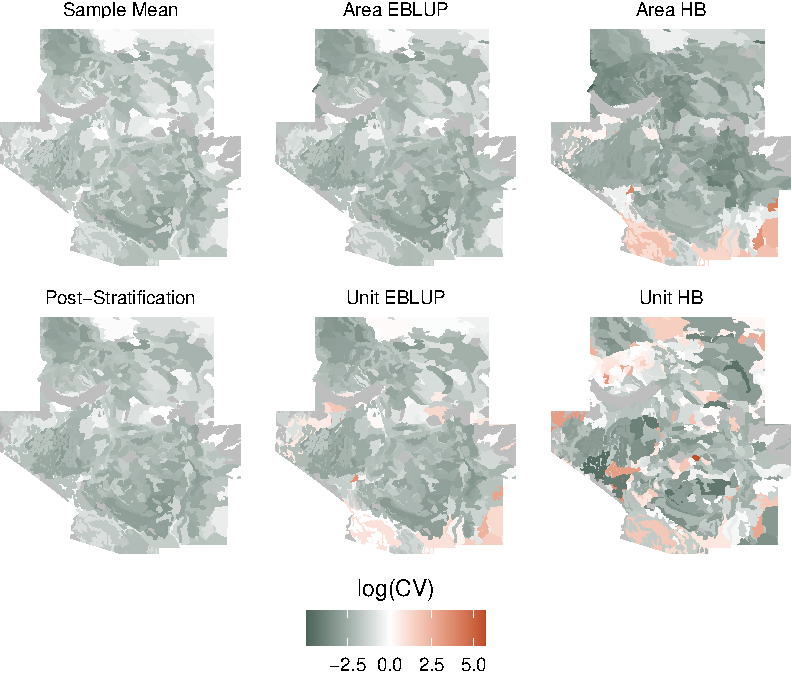
\includegraphics{thesis_files/figure-latex/cv-map-1} 

}

\caption[Coefficient of variation map]{Average log coefficient of variation of each estimator in each eco-subsection plotted onto a map of the Interior West. The average is taken over the four response variables. The natural log is used to perserve a reasonable color scale. Gray areas represent areas where models were not fit.}\label{fig:cv-map}
\end{figure}
The three estimators which have coefficient of variation values higher than one generally produce these values in heavily deserted areas in the southern parts of the Interior West and some deserts in the northern parts of Nevada. It makes sense that these areas may truly have low values for the response variables given that the post-stratified estimator is doing its job correctly and the population totals for forested and non-forested areas are correct. On the other hand, it may be reasonable to use a higher variance estimate in these cases and borrow strength from surrounding areas. While it is difficult to say which approach to handling these situations provides a better estimate, Figure \ref{fig:cv-map} highlights distinct ways in which the hierarchical Bayesian estimators (and the unit-level EBLUP) perform differently than the direct estimators and area-level EBLUP.
\clearpage

\hypertarget{zooming-in-the-northern-rocky-forest}{%
\section{Zooming In: The Northern Rocky Forest}\label{zooming-in-the-northern-rocky-forest}}

In order to take a closer look at \emph{how} borrowing of strength differs between the area-level hierarchical Bayesian estimator and the area-level EBLUP estimator, I chose to zoom in to basal area in the Northern Rocky Forest. Figure \ref{fig:m333-basal} displays the post-stratified, area-level EBLUP, and area-level hierarchical Bayesian estimates of basal area in the Northern Rocky Forest.
\begin{figure}

{\centering \includegraphics[width=1\linewidth]{thesis_files/figure-latex/m333-basal-1} 

}

\caption[Post-stratified, area-level EBLUP, and area-level HB estimates in M333]{The post-stratified estimator, frequentist area-level estimator, and the hierarchical Bayesian area-level estimator predicting basal area in the Northern Rocky Forest. The error bars depict two standard errors above and below the estimate of the response variable.}\label{fig:m333-basal}
\end{figure}
Immediately, when examining basal area in the Northern Rocky Forest, one can see the behavior of the hierarchical Bayesian area-level estimator ``pulling up'' lower valued eco-subsections compared to their post-stratified estimate. One can also observe that the eco-subsections with high response variable values will get ``pulled down.'' However, the coefficient of variation does not increase significantly here, as the sample mean is still relatively high. The pulling up and down of estimates is a trait expected of these hierarchical Bayesian models, and it is the realization of ``borrowing strength'' or ``pooling information'' (McElreath, 2020).

Figure \ref{fig:m333-basal} also displays the frequentist area-level estimator taking a different approach to making these estimates. Overall, the frequentist area-level estimator performs much more similarly to the post-stratified estimator, a trait that may or may not be appealing based on the confidence one has in the sampling process. However, it is important to note that the frequentist area-level estimator is still borrowing strength; it just appears that it will often borrow less strength than the hierarchical Bayesian area-level estimator. This is expected. Recall Equation \eqref{eq:eblup-area-weight} and note that when a large proportion of the total variation is between-area variation, the area-level EBLUP will rely heavily on the post-stratified estimate. Thus, in eco-subsections with low within-area variation, the area-level EBLUP will produce an estimate very similar to the post-stratified estimate. It is important to recall that much of the data contains many observations which equal zero (Figure \ref{fig:hists} and Table \ref{tab:var-tab}). So, in eco-subsections with a low number of sampled plots and a high proportion of sampled plots with response values equal to zero, artificially low variance may occur. The hierarchical Bayesian estimators have the unique property of considering the uncertainty in the variance estimate when producing estimates rather than relying on just a point value.

\hypertarget{stepping-back}{%
\section{Stepping Back}\label{stepping-back}}

When vision is narrowed to the Northern Rocky Forest, it does appear that the area-level hierarchical Bayesian estimator clearly outperforms the analogous frequentist estimator in all dimensions. However, I will now return to the Interior West in order to understand trends of estimator performance over space. To do this, I examine the eco-subsections in which the area-level hierarchical Bayesian estimator has lower variance than the post-stratified estimator and the area-level EBLUP in Figure \ref{fig:boolmap1}.
\clearpage
\begin{figure}

{\centering \includegraphics{thesis_files/figure-latex/boolmap1-1} 

}

\caption[Area-level coefficient of variation comparison across the Interior West]{The area-level hierarchical Bayesian estimator's coefficient of variation compared with the coefficient of variation for the post-stratified estimator (left) and area-level EBLUP (right). These are the average coefficient of variation across the four response variables studied. Eco-subsections in seafoam indicate areas in which the coefficient of variation is lower for the area-level hierarchical Bayesian estimator. Red areas indicate that the coefficient of variation of the hierarchical Bayesian estimator is greater than the estimator to which it is compared. Gray areas indicate areas in which we these estimators were not fit.}\label{fig:boolmap1}
\end{figure}
Generally, one is able to see the trend in Figure \ref{fig:cv-map} in which the area-level hierarchical Bayesian estimator produces estimates with higher variance in heavily deserted areas such as the southern parts of the Interior West and deserts in parts of Nevada. The areas in which the area-level hierarchical Bayesian estimator has more variation than the post-stratified estimator and the area-level EBLUP are clearly non-randomly distributed across the Interior West. This gives a great insight as to when one may want to use this hierarchical Bayesian estimator and further supports the idea that the area-level hierarchical Bayesian estimator has a high coefficient of variation in non-forested areas. These estimates are of the average coefficient of variation across our four response variables for each eco-subsection, and notably in 83.5\% and 82.5\% of these areas there is a decrease in the average coefficient of variation from the area-level hierarchical Bayesian estimator to the post-stratified estimator and the area-level EBLUP, respectively.

I have largely discussed the variance of these estimators thus far, as the true bias of an estimator cannot be known without knowing the population parameters \(\mu_{y_j}\) in each eco-subsection. However, in an attempt to quantify the magnitude of difference between two estimators, I introduce percent relative difference, which is defined below:
\begin{align*}
PRD(\hat\mu_1,~ \hat\mu_2) = \frac{\hat \mu_1 - \hat\mu_2}{\hat\mu_2} \cdot 100
\end{align*}
While one could explore percent relative difference among all combinations of estimators, the Forest Inventory and Analysis Program's go-to estimator is post-stratification. So I will compare the remaining five estimators to post-stratification. Additionally, post-stratification, as discussed in Chapter \ref{methods}, is an unbiased estimator given assumptions about the auxiliary data. Thus, I will rely on it for some proxy of truth. However, it is important to realize that this proxy is quite weak. Table \ref{tab:prd-tab} display the quantiles of percent relative difference to post-stratification.
\begin{longtable}[t]{lrrrrr}
\caption{\label{tab:prd-tab}Quantiles of Percent Relative Difference to the Post-Stratified Estimator}\\
\toprule
Estimator & 0\% & 25\% & 50\% & 75\% & 100\%\\
\midrule
Sample Mean & -60.997 & -3.826 & 0.056 & 5.610 & 1102.114\\
Unit HB & -99.928 & 1.326 & 21.816 & 94.770 & 24224.087\\
Area HB & -74.491 & -13.192 & 13.095 & 66.254 & 105994.261\\
Unit EBLUP & -80.319 & 3.521 & 25.471 & 99.885 & 27724.471\\
Area EBLUP & -79.641 & -3.747 & -0.165 & 2.802 & 160.843\\
\bottomrule
\end{longtable}
These quantiles continue to enforce the idea that the area-level EBLUP generally performs very similarly to the post-stratified estimator (albeit with lower variance). Notably, though, the percent relative difference between the area-level hierarchical Bayesian estimator and the post-stratified estimator is small compared to both unit-level models. The median values (50\% quantile) in Table \ref{tab:prd-tab} can be thought of as some sort of proxy for each estimator's bias, but this is a difficult equivalency to make when the parameter values are not available. While this proxy for bias may be weak, it is reassuring that for the area-level hierarchical Bayesian estimator, the median percent relative difference is somewhat low compared to other common estimators.

Another aspect of the results in this thesis that percent relative difference allows one to investigate is the performance of an estimator which I have hardly addressed so far: the hierarchical Bayesian unit-level model. This thesis claims to be a hierarchical Bayesian approach to small area estimation, yet the performance of one of the hierarchical Bayesian estimators has yet to be discussed in depth in this chapter. This is because the area-level hierarchical Bayesian estimator outperforms it by a huge margin in terms of variance. However, the case of the unit-level hierarchical Bayesian estimator is interesting in itself, even if it does not increase precision of estimates. To understand its performance, Table \ref{tab:prd-unit} examines its percent relative difference to the unit-level EBLUP estimator.
\begin{longtable}[t]{lrrrrr}
\caption{\label{tab:prd-unit}Quantiles of Percent Relative Difference to the Unit-level EBLUP}\\
\toprule
Estimator & 0\% & 25\% & 50\% & 75\% & 100\%\\
\midrule
Unit HB & -99.845 & -2.736 & -0.658 & -0.119 & 4.844\\
\bottomrule
\end{longtable}
One can immediately see that the unit-level hierarchical Bayesian estimator is extremely similar to the unit-level EBLUP. That is, many of their estimates are within just a few percent difference compared to the unit-level EBLUP. This is because the likelihood outweighs any prior information given to this model to a large degree. At the unit level, there are so many observations that any reasonable prior has a negligible effect on the estimator's results. This illustrates the idea that under ``flat'' or ``uninformative'' priors, the hierarchical Bayesian estimates will converge to the analogous EBLUP estimator's estimates. Also, recall that not only should the estimates converge to the same point, but the variance should, as well. I illustrate this in Figure \ref{fig:cov-violin} and in Figure \ref{fig:boolmap2} below.
\clearpage
\begin{figure}

{\centering \includegraphics{thesis_files/figure-latex/boolmap2-1} 

}

\caption[Unit-level coefficient of variation comparison across the Interior West]{The unit-level hierarchical Bayesian estimator's coefficient of variation compared with the coefficient of variation for the post-stratified estimator (left) and unit-level EBLUP (right). These are the average coefficient of variation across the four response variables studied. Eco-subsections in seafoam indicate areas in which the coefficient of variation is lower for the unit-level hierarchical Bayesian estimator. Red areas indicate that the coefficient of variation of the hierarchical Bayesian estimator is greater than the estimator to which it is compared. Gray areas indicate areas in which we these estimators were not fit.}\label{fig:boolmap2}
\end{figure}
The distribution of areas in which the hierarchical Bayesian unit-level estimator has lower variance than the unit-level EBLUP appears to be very random. Just under 46\% of areas have the hierarchical Bayesian unit-level model with lower variance than the unit-level EBLUP. In the case of this thesis, significant variance gains by implementing the unit-level hierarchical Bayesian estimator are not made; however, there are benefits of the implementation of this estimator. First, this piece of this thesis can serve as a case study of a hierarchical Bayesian estimator converging in variance and estimates to the analogous frequentist estimator. This allows for the verification of a statement often made in Bayesian statistics courses and textbooks with a real world example rather than a mathematical proof. Second, the unit-level hierarchical Bayesian estimator is much more flexible than the unit-level EBLUP and it does a very similar job to the unit-level EBLUP. One can ``tweak'' the behavior of this estimator through the use of priors, or even a different linking model if preferred. These changes could allow for a more successful estimator at the unit-level without changing many processes computationally. If one were to attempt to approach improving the unit-level model starting with the EBLUP, they would be met with restrictions due to the rigidity of the EBLUP's mathematics, and they would have to construct a new estimator entirely.

\hypertarget{discussion}{%
\chapter{Discussion}\label{discussion}}

\hypertarget{findings-and-takeaways}{%
\section{Findings and Takeaways}\label{findings-and-takeaways}}

I have introduced, fit, and presented the results of six small area estimators across the Interior West with four forestry-related response variables. Particularly, I introduced two estimators which are uncommon in forestry research: the hierarchical Bayesian unit- and area-level estimators. The area-level hierarchical Bayesian estimator reduces variance in estimates significantly compared to common direct estimators, frequentist model-based approaches (EBLUPs), and the unit-level hierarchical Bayesian estimator. There is a large reduction in variance compared to the area-level frequentist estimator and post-stratification in the great majority of small areas when implementing the hierarchical Bayesian area-level estimator. In extremely non-forested small areas, the hierarchical Bayesian area-level estimator consistently has higher variance than post-stratification or the area-level EBLUP. This is likely due to the way in which the area-level hierarchical Bayesian estimator borrows strength.

The area-level hierarchical Bayesian estimator produces very promising, low variance results in the Interior West, particularly in forested areas. Due to this trait, I believe that if this estimator was applied to data in the Pacific Northwest or Alaska, it may reduce variance even more than it did in the Interior West region. The unit-level hierarchical Bayesian estimator produces very similar estimates to the unit-level EBLUP; however, modifications to this estimator discussed later in this chapter could allow for a further reduction in variance.

\hypertarget{limitations}{%
\section{Limitations}\label{limitations}}

I now consider the scope of the research done in this thesis. While I broadly applied hierarchical Bayesian small area estimators across the Interior West, I also dealt with some small areas where the estimators produced NAs. This was due to either the hierarchical Bayesian unit- or area-level estimator producing errors when including these small areas in their estimation. After spending a great deal of time investigating which areas would produce these errors, I found that it was almost entirely areas which only had zero values for their response variables (or only a tiny number of plots which had non-zero response values). When aggregating the data to the area-level, tiny initial within-area variances for these estimators were calculated, which produced an error in the integration when computing the estimates. This is a limitation of numerical integration as a means towards a posterior distribution and the \texttt{hbsae} package, not one of the application of hierarchical Bayesian models for small area estimation. Using an R package such as \texttt{rstanarm} to compute the results would mitigate this problem, as MCMC methods would be used to attain our posterior (Goodrich, Gabry, Ali, \& Brilleman, 2020). It is important to remember that while this limitation is one of numerical integration and \texttt{hbsae}, there is a limitation in understanding the scope of the results fully without attaining estimates in every small area within the Interior West.

Another limitation of the research done in this thesis is the lack of population data for response variables. Without knowing the true mean of the response variables in eco-subsections of interest, it is difficult to understand how much bias each estimator is implementing. Attaining population data for any of the response variables in even one eco-subsection would be extremely expensive and impractical. However, a simulation study could be done to help understand bias of these estimators. This is discussed further in the following subsection.

\hypertarget{possible-extensions}{%
\section{Possible Extensions}\label{possible-extensions}}

Now I turn to possible extensions to the work which has been done in this thesis. I explore ideas for further research on adjacent topics and possibilities for applying these methods in other locations.

First, attempting to understand the performance of these hierarchical Bayesian estimators outside of the Interior West region of the United States through implementing these methods across the country would be insightful to the generalization of these estimators. Outside of the Interior West, the Forest Inventory and Analysis Programs has research stations in the Pacific Northwest region, Northern region, and Southern region. The hierarchical Bayesian area-level estimator is also a great candidate for estimation in Alaska. The reasons for its great candidacy are twofold: first, it is expensive and difficult to send foresters to collect data in Alaska due to the extreme rurality of the area; second, Alaska is very forested, and one thus would likely see a large reduction in variance of estimates when using the hierarchical Bayesian area-level estimator. The area-level hierarchical Bayesian estimator reduced variance in forested areas quite well, and applying this technique to data in Alaska could help mitigate the smaller sample size.

Another possibility for extending the research done in this thesis would be to adapt these hierarchical Bayesian estimators to produce estimates with lower variance under a variety of conditions. First, an implementation of a hybrid estimator could mitigate high variance in heavily non-forested areas. A hybrid estimator including both area-level model-based estimators which relies on the EBLUP's estimates in less-forested areas and the hierarchical Bayesian's estimates in more forested areas might result in lower variance across the board. The small areas in which the area-level hierarchical Bayesian estimator had higher variance than the area-level EBLUP were clearly non-random. A further analysis of these areas could lead to an insightful weighting system for this hybrid estimator. Another approach to mitigating the high variance seen in some eco-subsections for the area-level hierarchical Bayesian model would be to borrow strength differently, either through an explicit spatial analysis or by borrowing less strength (potentially to the eco-section level). Either of these methods could help weight areas closer to the eco-subsection of interest higher, potentially avoiding borrowing strength ``too far out'' that is potentially not strongly correlated with values in the eco-subsection of interest. Another way to mitigate this problem would be to introduce new auxiliary data. Auxiliary data which classifies the proportion of each eco-subsection that is a desert may help reduce variance in the more heavily-deserted eco-subsections.

An approach to more deeply understand the performance of these hierarchical Bayesian estimators would be to create a simulation study in which data are generated from known distributions. This would allow one to know the parameter values of \(\mu_{y_j}\), and one could better quantify the bias introduced by these estimators. This would be a great research project for a thesis student and would greatly help in the understanding of the overall performance of these estimators.

Finally, another large project worth exploring would be to embark on the development, testing, and documenting of a new R software package which would allow for more flexible hierarchical Bayesian small area estimators. The package used in this thesis, \texttt{hbsae}, has some nice features, such as its speed, due to the use of numerical integration rather than sampling from the posterior using Markov Chain Monte Carlo methods. However, this limits one's choice of functional forms of the distributions used in the estimators. With \texttt{hbsae}, one is limited to Inverse-Gamma distributions on the prior for variability, and more importantly, Gaussian response. The unit-level hierarchical Bayesian estimator may produce estimates with lower variance given that one models its response variable as something right-skewed: potentially either a Gamma distribution or a Tweedie distribution. The Tweedie distribution is often used in generalized linear modeling for data which are zero-inflated (Jorgensen, 1997). This makes it a great candidate for modeling the response variable of unit-level estimators. Outside of gaining flexibility, implementing new software with better documentation, consistent updates/patches, and a user-friendly manual would allow for researchers to implement these hierarchical Bayesian small area estimators more broadly and with ease.

\appendix

\hypertarget{code-appendix}{%
\chapter{Code Appendix}\label{code-appendix}}

This appendix includes the code used to create the estimates used in this thesis. Both the helper functions created to run the analyses and the implementation of these helper functions are included.

\hypertarget{helper-functions}{%
\section{Helper Functions}\label{helper-functions}}

\hypertarget{the-sample-mean}{%
\subsection{The Sample Mean}\label{the-sample-mean}}
\begin{verbatim}
direct_estimate <- function(data, response, small_area) {
  # Load packages
  library(sae)
  
  # Create dataframe
  dat <- data.frame(
    y = data[[response]],
    small_area = data[[small_area]]
  )
  
  # Compute estimate
  sae::direct(y = dat$y,
              dom = dat$small_area,
              replace = TRUE)
}
\end{verbatim}
\hypertarget{post-stratification}{%
\subsection{Post-Stratification}\label{post-stratification}}
\begin{verbatim}
postStrat2_bio <- function(data, strata) {
  est <- mase::postStrat(y = data[["BIOLIVE_TPA"]],
                  x_sample = data[["FIAstrat"]],
                  x_pop = strata,
                  data_type = "totals",
                  var_est = T)
  return(data.frame(ps_est = est$pop_mean,
                    sd = sqrt(est$pop_mean_var)))
}
postStrat2_ba <- function(data, strata) {
  est <- mase::postStrat(y = data[["BALIVE_TPA"]],
                  x_sample = data[["FIAstrat"]],
                  x_pop = strata,
                  data_type = "totals",
                  var_est = T)
  return(data.frame(ps_est = est$pop_mean,
                    sd = sqrt(est$pop_mean_var)))
}

postStrat2_voln <- function(data, strata) {
  est <- mase::postStrat(y = data[["VOLNLIVE_TPA"]],
                  x_sample = data[["FIAstrat"]],
                  x_pop = strata,
                  data_type = "totals",
                  var_est = T)
  return(data.frame(ps_est = est$pop_mean,
                    sd = sqrt(est$pop_mean_var)))
}

postStrat2_cnt <- function(data, strata) {
  est <- mase::postStrat(y = data[["CNTLIVE_TPA"]],
                  x_sample = data[["FIAstrat"]],
                  x_pop = strata,
                  data_type = "totals",
                  var_est = T)
  return(data.frame(ps_est = est$pop_mean,
                    sd = sqrt(est$pop_mean_var)))
}
\end{verbatim}
\hypertarget{hierarchical-bayesian-unit-level}{%
\subsection{Hierarchical Bayesian Unit-Level}\label{hierarchical-bayesian-unit-level}}
\begin{verbatim}
hb_unit <- function(data, formula, small_area, pop_data) {
  # Load packages
  library(tidyverse)
  library(hbsae)
  
  # Create model frame
  model_frame <- model.frame(formula, data) %>%
    dplyr::mutate(small_area = data[[small_area]])
  colnames(model_frame) <- c("y", "x", "small_area")
  
  # Area population sizes
  pop_size <- pop_data %>%
    dplyr::filter(zoneid %in% model_frame$small_area) %>%
    dplyr::select(zoneid, sum) %>%
    dplyr::rename(pop_size = sum) %>%
    dplyr::select(pop_size)
  
  # Create population means matrix
  pop_means <- pop_data %>%
    dplyr::filter(zoneid %in% model_frame$small_area) %>%
    dplyr::select(zoneid, mean) %>%
    dplyr::rename(x = mean) %>%
    column_to_rownames("zoneid")
  
  # Create lambda
  anova <- aov(y ~ small_area, data = model_frame)
  l <- summary(anova)[[1]]["small_area", "F value"]
  
  # Fit the model
  mod <- fSAE.Unit(
    y = model.frame(formula, data = data)[, 1],
    X = data.frame(X = model.frame(formula, data = data)[,-1]),
    area = data[[small_area]],
    Narea = pop_size$pop_size,
    Xpop = pop_means,
    fpc = TRUE,
    lambda0 = l,
    silent = T
  )

  # Calculate CoV
  mean_y <- model_frame %>%
    dplyr::group_by(small_area) %>%
    dplyr::summarise(mean_y = mean(y))
  CoV <- hbsae::SE(mod) / mean_y$mean_y

  ## Add to model object
  mod$CoV <- CoV

  # Print model
  mod
}
\end{verbatim}
\hypertarget{hierarchical-bayesian-area-level}{%
\subsection{Hierarchical Bayesian Area-Level}\label{hierarchical-bayesian-area-level}}
\begin{verbatim}
hb_area <- function(data, formula, small_area,
                    pop_data, post_strat_data) {
  # Load packages
  library(tidyverse)
  library(hbsae)
  
  # Create unnamed model frame (to call correct y var in a filter)
  mf <- model.frame(formula, data)
  
  # Create model frame
  model_frame <- model.frame(formula, data) %>%
    dplyr::mutate(small_area = data[[small_area]])
  colnames(model_frame) <- c("y", "x", "small_area")
  
  # Direct X
  X <- pop_data %>%
    dplyr::filter(zoneid %in% model_frame$small_area) %>%
    dplyr::select(zoneid, mean) %>%
    dplyr::rename(mean_x = mean,
                  small_area = zoneid) %>%
    dplyr::arrange(small_area)

  # Compute direct estimate
  mean <- direct_estimate(model_frame, "y", "small_area") %>%
    dplyr::mutate(var = SD^2)
  
  dir <- post_strat_data %>%
    filter(response %in% colnames(mf)[1],
           province %in% unique(data$province)) %>%
    arrange(subsection)
  
  # Create lambda
  anova <- aov(y ~ small_area, data = model_frame)
  l <- summary(anova)[[1]]["small_area", "F value"]

  # Fit the model
  mod <- fSAE.Area(
    est.init = dir$est,
    var.init = dir$var,
    X = X %>% dplyr::select(mean_x),
    lambda0 = l
  )

  # Calculate CoV
   CoV <- hbsae::SE(mod) / mean$Direct
   mod$CoV <- CoV

  # Print model
  mod
}
\end{verbatim}
\hypertarget{frequentist-unit-level}{%
\subsection{Frequentist Unit-Level}\label{frequentist-unit-level}}
\begin{verbatim}
freq_unit <- function(data, formula, small_area, pop_data) {
  # Load packages
  library(tidyverse)
  library(sae)
  
  # Create model frame
  model_frame <- model.frame(formula, data) %>%
    dplyr::mutate(small_area = data[[small_area]])
  colnames(model_frame) <- c("y", "x", "small_area")
  
  # Area population sizes
  pop_size <- pop_data %>%
    dplyr::filter(zoneid %in% model_frame$small_area) %>%
    dplyr::select(zoneid, sum) %>%
    dplyr::rename(pop_size = sum,
                  small_area = zoneid)
  
  # Create population means matrix
  meanxpop <- pop_data %>%
    dplyr::filter(zoneid %in% model_frame$small_area) %>%
    dplyr::select(zoneid, mean) %>%
    dplyr::rename(x = mean,
                  small_area = zoneid)
  
  # Fit the model
  mod <- eblupBHF(
    formula = model_frame$y ~ model_frame$x,
    dom = model_frame$small_area,
    meanxpop = meanxpop,
    popnsize = pop_size
  )
  mod
}
\end{verbatim}
\hypertarget{frequentist-area-level}{%
\subsection{Frequentist Area-Level}\label{frequentist-area-level}}
\begin{verbatim}
freq_area <- function(data, formula, small_area,
                      pop_data, post_strat_data) {
  # Load packages
  library(tidyverse)
  library(sae)
  
  # Create model frame
  model_frame <- model.frame(formula, data) %>%
    dplyr::mutate(small_area = data[[small_area]])
  colnames(model_frame) <- c("y", "x", "small_area")
  model_frame
  
  mf <- model.frame(formula, data)
  
  dir <- post_strat_data %>% 
    filter(response %in% colnames(mf)[1],
           province %in% unique(data$province)) %>%
    arrange(subsection)
  
  # Direct X
  X <- pop_data %>%
    dplyr::filter(zoneid %in% model_frame$small_area) %>%
    dplyr::select(zoneid, mean) %>%
    dplyr::rename(mean_x = mean,
                  small_area = zoneid) %>%
    dplyr::arrange(small_area)
  
  # Join pop and dir
  dat <- dir %>%
    left_join(X, by = c("subsection" = "small_area"))

  # Fit the model
  mod <- sae::mseFH(formula = dat$est ~ dat$mean_x,
                      vardir = dat$var)
  mod
  
}
\end{verbatim}
\hypertarget{coeffiicent-of-variation-functions}{%
\subsection{Coeffiicent of Variation Functions}\label{coeffiicent-of-variation-functions}}
\begin{verbatim}
hb_CoV <- function(data) {
  # Load packages
  library(tidyverse)
  library(hbsae)
  
  # Grab CoV
  data$CoV
}

freq_unit_CoV <- function(data, formula, small_area,
                          pop_data, B = 100) {
  # Load packages
  library(tidyverse)
  library(sae)
  
  # Create empty items for looping
  boots <- list()
  fit <- list()
  mean_df <- list()
  final <- data.frame()
  
  # Create model frame
  model_frame <- model.frame(formula, data) %>%
    dplyr::mutate(small_area = data[[small_area]])
  colnames(model_frame) <- c("y", "x", "small_area")
  
  # Nest by small area
  data_nested <- model_frame %>%
    mutate(id = small_area) %>%
    group_by(small_area) %>%
    nest()
  
  # Bootstrap
  for(i in 1:B){
    for(j in 1:length(unique(model_frame$small_area))) {
      boots[[j]] <- sample_n(
        data_nested[[2]][[j]],
        size = length(data_nested[[2]][[j]]$y),
        replace = TRUE
      )
      boots_df <- bind_rows(boots) 
    }
    
    fit[[i]] <- freq_unit(boots_df, y ~ x, "id", pop_data)
    
    mean_df[[i]] <- data.frame(fitted = fit[[i]]$eblup$eblup,
                               subsection = fit[[i]]$eblup$domain)
    if (i %% 50 == 1) {
      print(i)
    }
  }
  
  # Create final output
  final <- bind_rows(mean_df) %>%
    group_by(subsection) %>%
    summarize(sd = sd(fitted, na.rm = TRUE))
  mean_y <- model_frame %>%
    dplyr::group_by(small_area) %>%
    dplyr::summarise(mean_y = mean(y, na.rm = TRUE))
  
  COV <- final$sd / mean_y$mean_y
  names(COV) <- final$subsection
  
  COV
}
\end{verbatim}
\hypertarget{fitting-models}{%
\section{Fitting Models}\label{fitting-models}}

\hypertarget{data-set-up-preprocessing}{%
\subsection{Data Set-up \& Preprocessing}\label{data-set-up-preprocessing}}
\begin{verbatim}
library(tidyverse)
library(mase)
library(hbsae)
library(sae)
\end{verbatim}
\begin{verbatim}
intwest <- read_csv("data/subsets/df.csv")
tccpop <- read_csv("data/population/tcc_pop.csv")
strata <- read_csv("data/population/strata.csv")
\end{verbatim}
\begin{verbatim}
# Set-up strata:
intwest <- intwest %>%
  mutate(FIAstrat = case_when(
    FIAstrat == "1" ~ "Sampled-Forest",
    FIAstrat == "2" ~ "Sampled-Nonforest",
    FIAstrat == "0" ~ "Sampled-Nonforest",
    FIAstrat == "3" ~ "Sampled-Nonforest",
  )) 
\end{verbatim}
\begin{verbatim}
# Filter out subsections that cause errors in computation
no0_subsections <- intwest %>%
  group_by(subsection) %>%
  summarize(mean_y = mean(BIOLIVE_TPA),
            mean_x = mean(nlcd11)) %>%
  filter(mean_y > 0 & mean_x > 0) %>% 
  dplyr::select(subsection) %>%
  pull()

intwest_no0 <- intwest %>%
  filter(subsection %in% no0_subsections) %>%
  filter(!(province %in% c("M261", "M334"))) %>% 
  filter(!(subsection %in% c("342Fi", "331Kj", "342Dh", "341Dc"))) 
\end{verbatim}
\begin{verbatim}
# Create list of dataframes
iw <- split(intwest_no0, f = intwest_no0$province)
\end{verbatim}
\hypertarget{direct-estimation-1}{%
\subsection{Direct Estimation}\label{direct-estimation-1}}
\begin{verbatim}
strata <- strata %>%
  filter(zoneid %in% unique(intwest_no0$subsection)) %>%
  mutate(
    fnf_no_water = case_when(
      fnf_no_water == 1 ~ "Sampled-Forest",
      fnf_no_water == 2 ~ "Sampled-Nonforest"
    )
  )
strata <- strata %>%
  dplyr::select(-zoneprop)

# split strata into list and drop column split by
strata_list <- lapply(
  split(strata, f = strata$zoneid),
  function(strata) { strata$zoneid <- NULL; strata}
  )

# split subsections into list
subsection_list <- split(intwest_no0,
                         intwest_no0$subsection)


post_strat_bio <- map2(.x = subsection_list,
                       .y = strata_list,
                       .f = postStrat2_bio)
post_strat_ba <- map2(.x = subsection_list,
                      .y = strata_list,
                      .f = postStrat2_ba)
post_strat_voln <- map2(.x = subsection_list,
                        .y = strata_list,
                        .f = postStrat2_voln)
post_strat_cnt <- map2(.x = subsection_list,
                       .y = strata_list,
                       .f = postStrat2_cnt)

results <- data.frame(
  ps_est = c(bind_rows(post_strat_bio)$ps_est,
             bind_rows(post_strat_ba)$ps_est,
             bind_rows(post_strat_cnt)$ps_est,
             bind_rows(post_strat_voln)$ps_est),
  ps_sd = c(bind_rows(post_strat_bio)$sd,
             bind_rows(post_strat_ba)$sd,
             bind_rows(post_strat_cnt)$sd,
             bind_rows(post_strat_voln)$sd),
  subsection = rep(names(post_strat_bio), 4),
  response = c(
    rep("BIOLIVE_TPA", length(post_strat_bio)),
    rep("BALIVE_TPA", length(post_strat_ba)),
    rep("CNTLIVE_TPA", length(post_strat_cnt)),
    rep("VOLNLIVE_TPA", length(post_strat_voln)))
)
\end{verbatim}
\begin{verbatim}
dirmean <- list()
dirmean[1:length(iw)] <- 
  lapply(iw,
         direct_estimate,
         response = "BIOLIVE_TPA", 
         "subsection")
dirmean[(length(iw) + 1):(2 * length(iw))] <- 
  lapply(iw,
        direct_estimate,
        response = "BALIVE_TPA",
        "subsection")
dirmean[(2*length(iw) + 1):(3*length(iw))] <- 
  lapply(iw,
         direct_estimate,
         response = "CNTLIVE_TPA",
         "subsection")
dirmean[(3*length(iw) + 1):(4*length(iw))] <- 
  lapply(iw,
         direct_estimate,
         response = "VOLNLIVE_TPA",
         "subsection")

dir <- bind_rows(dirmean) %>%
  dplyr::select(Domain, Direct, CV) %>%
  mutate(cov_dirmean = CV / 100) %>%
  rename(est_dirmean = Direct) %>%
  dplyr::select(-CV) %>%
  mutate(response = c(
    rep("BIOLIVE_TPA", length(post_strat_bio)),
    rep("BALIVE_TPA", length(post_strat_ba)),
    rep("CNTLIVE_TPA", length(post_strat_cnt)),
    rep("VOLNLIVE_TPA", length(post_strat_voln))))

results <- results %>%
  left_join(dir, by = c("subsection" = "Domain",
                        "response" = "response"))
\end{verbatim}
\begin{verbatim}
# Create CoV for ps-estimator
results <- results %>%
  mutate(
    cov_dirps = ps_sd / est_dirmean
  )

# change names and rearrange 
results <- results %>%
  rename(est_dirps = ps_est,
         sd_dirps = ps_sd) %>%
  relocate("subsection", "response",
           "est_dirps", "cov_dirps")
\end{verbatim}
\hypertarget{model-based-estimation}{%
\subsection{Model-Based Estimation}\label{model-based-estimation}}
\begin{verbatim}
# set up list for area level models
ps_dat <- results %>%
  dplyr::select(est_dirps, sd_dirps,
                subsection, response) %>%
  dplyr::mutate(var = sd_dirps^2) %>%
  dplyr::rename(est = est_dirps) %>%
  dplyr::select(est, var, subsection, response) %>%
  dplyr::mutate(
    section = str_remove_all(subsection, "[:lower:]"),
    province = str_sub(section, end = -2))

ps_l <- split(ps_dat, list(ps_dat$province))
\end{verbatim}
\begin{verbatim}
# HB Unit
set.seed(1)
bayes_unit <- list()
bayes_unit[1:length(iw)] <- lapply(
  iw,
  hb_unit,
  formula = BIOLIVE_TPA ~ nlcd11,
  small_area = "subsection",
  pop_data = tccpop
)
bayes_unit[(length(iw) + 1):(2 * length(iw))] <-
  lapply(
    iw,
    hb_unit,
    formula = BALIVE_TPA ~ nlcd11,
    small_area = "subsection",
    pop_data = tccpop
  )
bayes_unit[(2 * length(iw) + 1):(3 * length(iw))] <-
  lapply(
    iw,
    hb_unit,
    formula = CNTLIVE_TPA ~ nlcd11,
    small_area = "subsection",
    pop_data = tccpop
  )
bayes_unit[(3 * length(iw) + 1):(4 * length(iw))] <-
  lapply(
    iw,
    hb_unit,
    formula = VOLNLIVE_TPA ~ nlcd11,
    small_area = "subsection",
    pop_data = tccpop
  )

res_hbu <- data.frame(
  subsection = names(unlist(lapply(bayes_unit, EST))),
response = c(
    rep("BIOLIVE_TPA", length(post_strat_bio)),
    rep("BALIVE_TPA", length(post_strat_ba)),
    rep("CNTLIVE_TPA", length(post_strat_cnt)),
    rep("VOLNLIVE_TPA", length(post_strat_voln))),
  est_hb_unit = unlist(lapply(bayes_unit, EST)),
  cov_hb_unit = unlist(lapply(bayes_unit, hb_CoV))
)

results <- results %>%
  left_join(res_hbu, by = c("subsection" = "subsection",
                        "response" = "response"))
\end{verbatim}
\begin{verbatim}
# HB Area
set.seed(1)
bayes_area <- list()
bayes_area[1:length(iw)] <-
  lapply(
    iw,
    hb_area,
    formula = BIOLIVE_TPA ~ nlcd11,
    small_area = "subsection",
    pop_data = tccpop,
    post_strat_data = ps_dat
  )
bayes_area[(length(iw) + 1):(2 * length(iw))] <-
  lapply(
    iw,
    hb_area,
    formula = BALIVE_TPA ~ nlcd11,
    small_area = "subsection",
    pop_data = tccpop,
    post_strat_data = ps_dat
  )
bayes_area[(2 * length(iw) + 1):(3 * length(iw))] <-
  lapply(
    iw,
    hb_area,
    formula = CNTLIVE_TPA ~ nlcd11,
    small_area = "subsection",
    pop_data = tccpop,
    post_strat_data = ps_dat
  )
bayes_area[(3 * length(iw) + 1):(4 * length(iw))] <-
  lapply(
    iw,
    hb_area,
    formula = VOLNLIVE_TPA ~ nlcd11,
    small_area = "subsection",
    pop_data = tccpop,
    post_strat_data = ps_dat
  )

aranged_df <- intwest_no0 %>%
  filter(province %in% names(iw)) %>%
  arrange(province) %>%
  arrange(subsection)
hb_area_res <- data.frame(
  subsection = rep(unique(aranged_df$subsection), 4),
  est_hb_area = unlist(lapply(bayes_area, EST)),
  cov_hb_area = unlist(lapply(bayes_area, hb_CoV)),
  response = c(
    rep("BIOLIVE_TPA", length(post_strat_bio)),
    rep("BALIVE_TPA", length(post_strat_ba)),
    rep("CNTLIVE_TPA", length(post_strat_cnt)),
    rep("VOLNLIVE_TPA", length(post_strat_voln))
  )
)

results <- results %>%
  left_join(hb_area_res, by = c("subsection" = "subsection",
                                "response" = "response"))
\end{verbatim}
\begin{verbatim}
# Freq Unit
set.seed(1)
frequnit <- list()
frequnit[1:length(iw)] <-
  lapply(iw,
         freq_unit,
         formula = BIOLIVE_TPA ~ nlcd11,
         "subsection",
         tccpop)
frequnit[(length(iw) + 1):(2 * length(iw))] <-
  lapply(iw,
         freq_unit,
         formula = BALIVE_TPA ~ nlcd11,
         "subsection",
         tccpop)
frequnit[(2 * length(iw) + 1):(3 * length(iw))] <-
  lapply(iw, 
         freq_unit,
         formula = CNTLIVE_TPA ~ nlcd11,
         "subsection", 
         tccpop)
frequnit[(3 * length(iw) + 1):(4 * length(iw))] <-
  lapply(iw,
         freq_unit,
         formula = VOLNLIVE_TPA ~ nlcd11,
         "subsection",
         tccpop)

frequnit_list <- list()
  for(i in 1:(4 * length(iw))) {
    frequnit_list[[i]] <- frequnit[[i]]$eblup
  }

frequnit_df <- frequnit_list %>%
  bind_rows() %>%
  mutate(response = c(
    rep("BIOLIVE_TPA", length(post_strat_bio)),
    rep("BALIVE_TPA", length(post_strat_ba)),
    rep("CNTLIVE_TPA", length(post_strat_cnt)),
    rep("VOLNLIVE_TPA", length(post_strat_voln)))) %>%
  rename(
    subsection = domain,
    est_freq_unit = eblup
  ) %>%
  dplyr::select(-sampsize)

# Coef of variation
frequnitcov <- c()
frequnitcov <- c(
  Reduce(c,
       lapply(iw,
       freq_unit_CoV,
       formula = BIOLIVE_TPA ~ nlcd11,
       small_area = "subsection",
       pop_data = tccpop,
       B = 500)),
  Reduce(c,
       lapply(iw,
       freq_unit_CoV,
       formula = BALIVE_TPA ~ nlcd11,
       small_area = "subsection",
       pop_data = tccpop,
       B = 500)),
  Reduce(c,
       lapply(iw,
       freq_unit_CoV,
       formula = CNTLIVE_TPA ~ nlcd11,
       small_area = "subsection",
       pop_data = tccpop,
       B = 500)),
  Reduce(c,
       lapply(iw,
       freq_unit_CoV,
       formula = VOLNLIVE_TPA ~ nlcd11,
       small_area = "subsection",
       pop_data = tccpop,
       B = 500))
)

frequnitcov_df <- data.frame(
  cov_freq_unit = frequnitcov,
  subsection = names(frequnitcov),
  response = c(
    rep("BIOLIVE_TPA", length(post_strat_bio)),
    rep("BALIVE_TPA", length(post_strat_ba)),
    rep("CNTLIVE_TPA", length(post_strat_cnt)),
    rep("VOLNLIVE_TPA", length(post_strat_voln))
  )
)

frequnit_df <- frequnit_df %>%
  left_join(frequnitcov_df,
            by = c("subsection" = "subsection",
                   "response" = "response"))

results <- results %>%
  left_join(frequnit_df,
            by = c("subsection" = "subsection",
                   "response" = "response"))
\end{verbatim}
\begin{verbatim}
# Freq Area
set.seed(1)
freqarea <- list()
freqarea[1:length(iw)] <-
  lapply(
    iw,
    freq_area,
    formula = BIOLIVE_TPA ~ nlcd11,
    "subsection",
    tccpop,
    post_strat_data = ps_dat
)
freqarea[(length(iw) + 1):(2 * length(iw))] <- 
  lapply(
    iw,
    freq_area,
    formula = BALIVE_TPA ~ nlcd11,
    "subsection",
    tccpop,
    post_strat_data = ps_dat
)
freqarea[(2 * length(iw) + 1):(3 * length(iw))] <-
  lapply(
    iw,
    freq_area,
    formula = CNTLIVE_TPA ~ nlcd11,
    "subsection",
    tccpop,
    post_strat_data = ps_dat
)
freqarea[(3 * length(iw) + 1):(4 * length(iw))] <-
  lapply(
    iw,
    freq_area,
    formula = VOLNLIVE_TPA ~ nlcd11,
    "subsection",
    tccpop,
    post_strat_data = ps_dat
)

freqarea_list <- list()
for (i in 1:(4 * length(iw))) {
  freqarea_list[[i]] <- freqarea[[i]]$est$eblup
}
freqarea_cov_list <- list()
for (i in 1:(4 * length(iw))) {
  freqarea_cov_list[[i]] <- sqrt(freqarea[[i]]$mse)
}

freq_area_res <- data.frame(
  subsection = rep(unique(aranged_df$subsection), 4),
  est_freq_area = unlist(freqarea_list),
  se_freq_area = unlist(freqarea_cov_list),
  response = c(
    rep("BIOLIVE_TPA", length(post_strat_bio)),
    rep("BALIVE_TPA", length(post_strat_ba)),
    rep("CNTLIVE_TPA", length(post_strat_cnt)),
    rep("VOLNLIVE_TPA", length(post_strat_voln))
  )
)
results <- results %>%
  left_join(freq_area_res,
            by = c("subsection" = "subsection",
                   "response" = "response"))
results <- results %>%
  mutate(cov_freq_area = se_freq_area / est_dirmean)
\end{verbatim}
\hypertarget{writing-data-files-pivoting-to-tidy-format}{%
\subsection{Writing Data Files \& Pivoting to Tidy Format}\label{writing-data-files-pivoting-to-tidy-format}}
\begin{verbatim}
write.csv(results, 
          "data/results/final_results.csv")
saveRDS(results,
        file = "data/results/final_results.rds")
\end{verbatim}
\begin{verbatim}
estimates_long <- results %>%
  pivot_longer(cols = c("est_hb_unit", "est_hb_area",
                        "est_freq_unit", "est_freq_area", 
                        "est_dirmean", "est_dirps"),
               names_to = "estimator",
               values_to = "estimate") %>%
  dplyr::select(-cov_hb_unit, -cov_hb_area,
                -cov_freq_unit, -cov_freq_area,
                -cov_dirmean, -cov_dirps) %>%
  mutate(estimator = stringr::str_sub(estimator, start = 5))

cov_long <- results %>%
  pivot_longer(cols = c("cov_hb_unit", "cov_hb_area",
                        "cov_freq_unit", "cov_freq_area",
                        "cov_dirmean", "cov_dirps"),
               names_to = "estimator",
               values_to = "cov") %>%
  dplyr::select(-est_hb_unit, -est_hb_area,
                -est_freq_unit, -est_freq_area,
                -est_dirmean, -est_dirps) %>%
  mutate(estimator = stringr::str_sub(estimator, start = 5))

final_results_long <- estimates_long %>%
  full_join(cov_long) %>%
  mutate(
    section = str_remove_all(subsection, "[:lower:]"),
    province = str_sub(section, end = -2)
  )

final_results_long <- final_results_long %>%
  dplyr::select(-sd_dirps, -se_freq_area)
\end{verbatim}
\begin{verbatim}
write.csv(final_results_long,
          "data/results/final_results_long.csv")
saveRDS(final_results_long,
        file = "data/results/final_results_long.rds")
\end{verbatim}
\backmatter

\hypertarget{references}{%
\chapter*{References}\label{references}}
\addcontentsline{toc}{chapter}{References}

\markboth{References}{References}

\noindent

\setlength{\parindent}{-0.20in}
\setlength{\leftskip}{0.20in}
\setlength{\parskip}{8pt}

\hypertarget{refs}{}
\begin{CSLReferences}{1}{0}
\leavevmode\vadjust pre{\hypertarget{ref-bayes-orig}{}}%
Bayes, T. (1763). LII. An essay towards solving a problem in the doctrine of chances. By the late rev. Mr. Bayes, FRS communicated by mr. Price, in a letter to john canton, AMFR s. \emph{Philosophical Transactions of the Royal Society of London}, (53), 370--418.

\leavevmode\vadjust pre{\hypertarget{ref-greenbook}{}}%
Bechtold, W. A., \& Patterson, P. L. (2005). \emph{The enhanced forest inventory and analysis program--national sampling design and estimation procedures} (Vol. 80). USDA Forest Service, Southern Research Station.

\leavevmode\vadjust pre{\hypertarget{ref-hbsae-package}{}}%
Boonstra, H. J. (2012). \emph{Hbsae: Hierarchical bayesian small area estimation}. Retrieved from \url{https://CRAN.R-project.org/package=hbsae}

\leavevmode\vadjust pre{\hypertarget{ref-andrew-392}{}}%
Bray, A. (2020). Math 392: Mathematical statistics.

\leavevmode\vadjust pre{\hypertarget{ref-breidenbach2012}{}}%
Breidenbach, J., \& Astrup, R. (2012). Small area estimation of forest attributes in the norwegian national forest inventory. \emph{European Journal of Forest Research}, \emph{131}(4), 1255--1267.

\leavevmode\vadjust pre{\hypertarget{ref-bootstrap}{}}%
Efron, B. (1992). Bootstrap methods: Another look at the jackknife. In \emph{Breakthroughs in statistics} (pp. 569--593). Springer.

\leavevmode\vadjust pre{\hypertarget{ref-whatisfia}{}}%
FIA. (2020). Forest inventory and analysis national program. \emph{What is FIA?} Retrieved from \url{https://www.fia.fs.fed.us/about/about_us/}

\leavevmode\vadjust pre{\hypertarget{ref-rstanarm}{}}%
Goodrich, B., Gabry, J., Ali, I., \& Brilleman, S. (2020). Rstanarm: {Bayesian} applied regression modeling via {Stan}. Retrieved from \url{https://mc-stan.org/rstanarm}

\leavevmode\vadjust pre{\hypertarget{ref-mse-area}{}}%
Hidiroglou, M., \& You, Y. (2016). Comparison of unit level and area level small area estimators, \emph{42}, 41--61.

\leavevmode\vadjust pre{\hypertarget{ref-nlcd11}{}}%
Homer, C. (2015, November). Completion of the 2011 national land cover database for the conterminous united states -- representing a decade of land cover change information. \emph{EPA}. Environmental Protection Agency. Retrieved from \url{https://cfpub.epa.gov/si/si_public_record_report.cfm?Lab=NERL\&dirEntryId=309950}

\leavevmode\vadjust pre{\hypertarget{ref-doves}{}}%
Hooten, M. B., \& Wikle, C. K. (2008). A hierarchical bayesian non-linear spatio-temporal model for the spread of invasive species with application to the eurasian collared-dove. \emph{Environmental and Ecological Statistics}, \emph{15}(1), 59--70.

\leavevmode\vadjust pre{\hypertarget{ref-hor52}{}}%
Horvitz, D. G., \& Thompson, D. J. (1952). A generalization of sampling without replacement from a finite universe. \emph{Journal of the American Statistical Association}, \emph{47}, 663--685.

\leavevmode\vadjust pre{\hypertarget{ref-inbook}{}}%
Iriawan, N., \& Yasmirullah, S. (2019). An economic growth model using hierarchical bayesian method. http://doi.org/\href{https://doi.org/10.5772/intechopen.88650}{10.5772/intechopen.88650}

\leavevmode\vadjust pre{\hypertarget{ref-jorgensen1997theory}{}}%
Jorgensen, B. (1997). \emph{The theory of dispersion models}. CRC Press.

\leavevmode\vadjust pre{\hypertarget{ref-mcconville2020}{}}%
McConville, K. S., Moisen, G. G., \& Frescino, T. S. (2020). A tutorial on model-assisted estimation with application to forest inventory. \emph{Forests}, \emph{11}(2).

\leavevmode\vadjust pre{\hypertarget{ref-mase}{}}%
McConville, K., Tang, B., Zhu, G., Cheung, S., \& Li, S. (2018). \emph{Mase: Model-assisted survey estimation}. Retrieved from \url{https://cran.r-project.org/package=mase}

\leavevmode\vadjust pre{\hypertarget{ref-statrethinking}{}}%
McElreath, R. (2020). \emph{Statistical rethinking: A bayesian course with examples in r and STAN}.

\leavevmode\vadjust pre{\hypertarget{ref-latex2exp}{}}%
Meschiari, S. (2021). \emph{latex2exp: Use LaTeX expressions in plots}. Retrieved from \url{https://CRAN.R-project.org/package=latex2exp}

\leavevmode\vadjust pre{\hypertarget{ref-sae-package}{}}%
Molina, I., \& Marhuenda, Y. (2015). {sae}: An {R} package for small area estimation. \emph{The R Journal}, \emph{7}(1), 81--98. Retrieved from \url{https://journal.r-project.org/archive/2015/RJ-2015-007/RJ-2015-007.pdf}

\leavevmode\vadjust pre{\hypertarget{ref-USAboundaries}{}}%
Mullen, L. A., \& Bratt, J. (2018). {USAboundaries}: Historical and contemporary boundaries of the united states of america. \emph{Journal of Open Source Software}, \emph{3}, 314. http://doi.org/\href{https://doi.org/10.21105/joss.00314}{10.21105/joss.00314}

\leavevmode\vadjust pre{\hypertarget{ref-sf}{}}%
Pebesma, E. (2018). {Simple Features for R: Standardized Support for Spatial Vector Data}. \emph{{The R Journal}}, \emph{10}(1), 439--446. http://doi.org/\href{https://doi.org/10.32614/RJ-2018-009}{10.32614/RJ-2018-009}

\leavevmode\vadjust pre{\hypertarget{ref-patchwork}{}}%
Pedersen, T. L. (2020). \emph{Patchwork: The composer of plots}. Retrieved from \url{https://CRAN.R-project.org/package=patchwork}

\leavevmode\vadjust pre{\hypertarget{ref-r-software}{}}%
R Core Team. (2020). \emph{R: A language and environment for statistical computing}. Vienna, Austria: R Foundation for Statistical Computing. Retrieved from \url{https://www.R-project.org/}

\leavevmode\vadjust pre{\hypertarget{ref-rao2014}{}}%
Rao, J. N. (2014). Small-area estimation. \emph{Wiley StatsRef: Statistics Reference Online}.

\leavevmode\vadjust pre{\hypertarget{ref-med}{}}%
Tojtovska, B., Ribarski, P., \& Ljubic, A. (2019). Application of hierarchical bayesian model in ophtalmological study. In S. Gievska \& G. Madjarov (Eds.), \emph{ICT innovations 2019. Big data processing and mining} (pp. 109--120). Cham: Springer International Publishing.

\leavevmode\vadjust pre{\hypertarget{ref-ver2017}{}}%
Ver Planck, N. R., Finley, A. O., \& Huff, E. S. (2017). Hierarchical bayesian models for small area estimation of county-level private forest landowner population. \emph{Canadian Journal of Forest Research}, \emph{47}(12), 1577--1589.

\leavevmode\vadjust pre{\hypertarget{ref-agri}{}}%
Wang, J. C., Holan, S. H., Nandram, B., Barboza, W., Toto, C., \& Anderson, E. (2012). A bayesian approach to estimating agricultural yield based on multiple repeated surveys. \emph{Journal of Agricultural, Biological, and Environmental Statistics}, \emph{17}(1), 84--106.

\leavevmode\vadjust pre{\hypertarget{ref-tidyverse}{}}%
Wickham, H., Averick, M., Bryan, J., Chang, W., McGowan, L. D., François, R., \ldots{} Yutani, H. (2019). Welcome to the {tidyverse}. \emph{Journal of Open Source Software}, \emph{4}(43), 1686. http://doi.org/\href{https://doi.org/10.21105/joss.01686}{10.21105/joss.01686}

\leavevmode\vadjust pre{\hypertarget{ref-scales}{}}%
Wickham, H., \& Seidel, D. (2020). \emph{Scales: Scale functions for visualization}. Retrieved from \url{https://CRAN.R-project.org/package=scales}

\end{CSLReferences}

% Index?

\end{document}
